%\clearpage
\fancyhead[LO,RE]{ANEXOS}
\appendix
\renewcommand{\appendixname}{Anexos}
\renewcommand{\appendixtocname}{Anexos}
\renewcommand{\appendixpagename}{Anexos}
\clearpage
\addappheadtotoc
%\appendixpage %Agrega una pagina en blanco q en el medio Dice Anexo en grande..



    \begin{minipage}{0.95\textwidth}
    \chapter{Diagrama del modelo de casos de uso}
    %\section{Diagrama del modelo de casos de uso}
    	\leftline{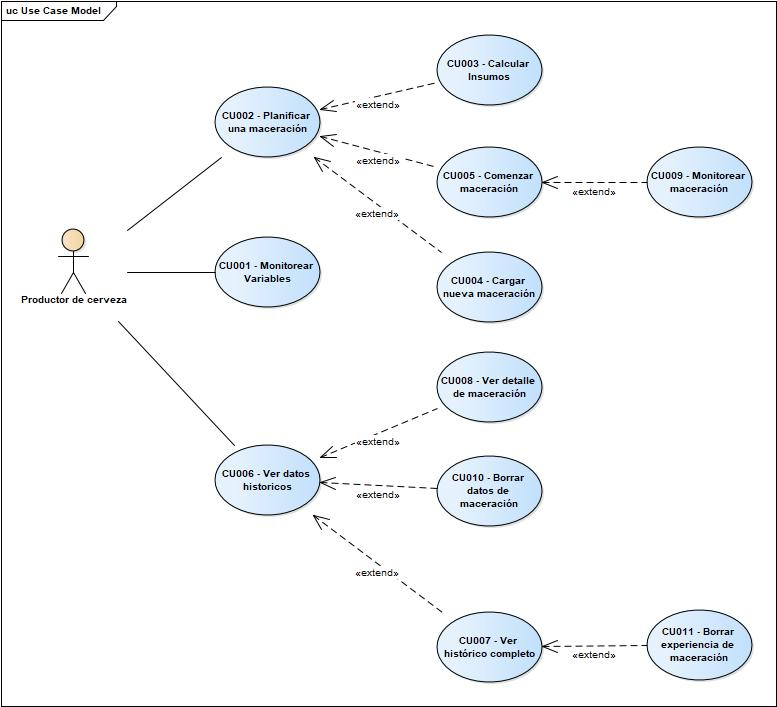
\includegraphics[scale=0.7]{ModelodeCasosdeUso.jpg}}
    	\captionof{figure}{Diagrama de Casos de Uso}
	    \label{DiagCU}
	\end{minipage}


    \begin{minipage}{0.95\textwidth}
    \chapter{Diagrama de base de datos del componente de hardware}
        \centering
        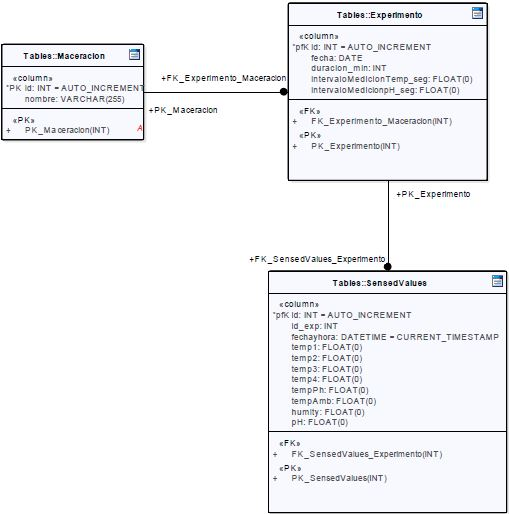
\includegraphics[scale=0.65]{diagramaBD-Rasp.jpg}
        \captionof{figure}{Diagrama de diseño de Base de Datos}
        \label{fig:DiagramaBdRasp}
    
    \end{minipage}
    
    \begin{minipage}{0.95\textwidth}
    \chapter{Esquema de conexión de la estación de recolección de datos}
        \centering
        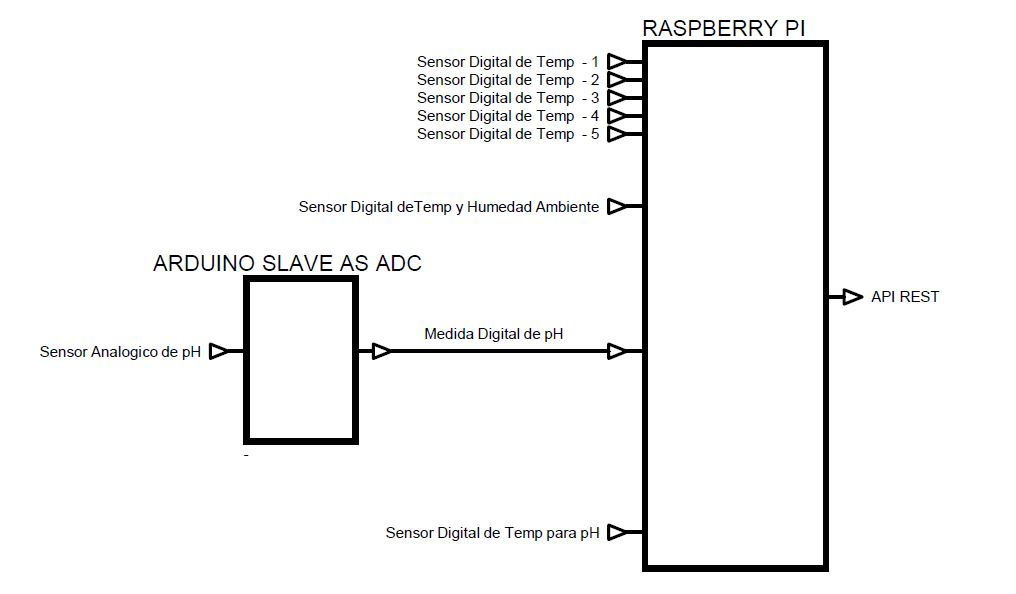
\includegraphics[scale=0.55]{EsquemaHardware.jpg}
        \captionof{figure}{Esquema simplificado de las conexiones}
        \label{fig:EsquemaHardware}
    \end{minipage}
    
%---------------------- MOCK UP ----------------------------------------
    \begin{minipage}{0.95\textwidth}
    \chapter{Diseño de interfaz de usuario}
    %\section{Diseño de Interfaz de Usuario}
        \centering
        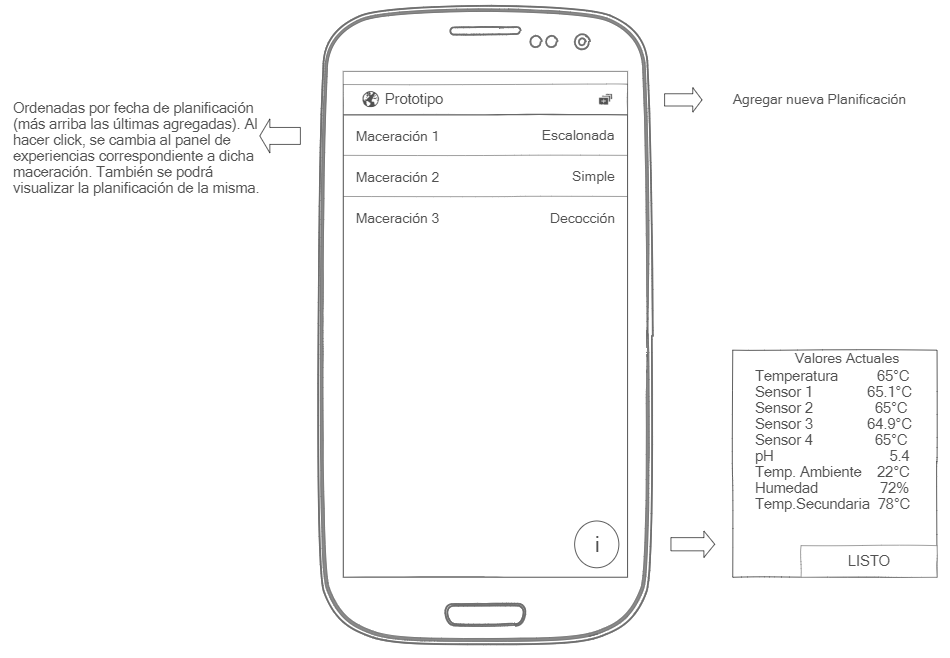
\includegraphics[scale=0.55]{Anexo/MockUp/MainActivity.jpg}
        \captionof{figure}{Pantalla Principal}
        \label{fig:MockUpMainActivity}
    \end{minipage}
    
    \begin{minipage}{0.95\textwidth}

        \centering
        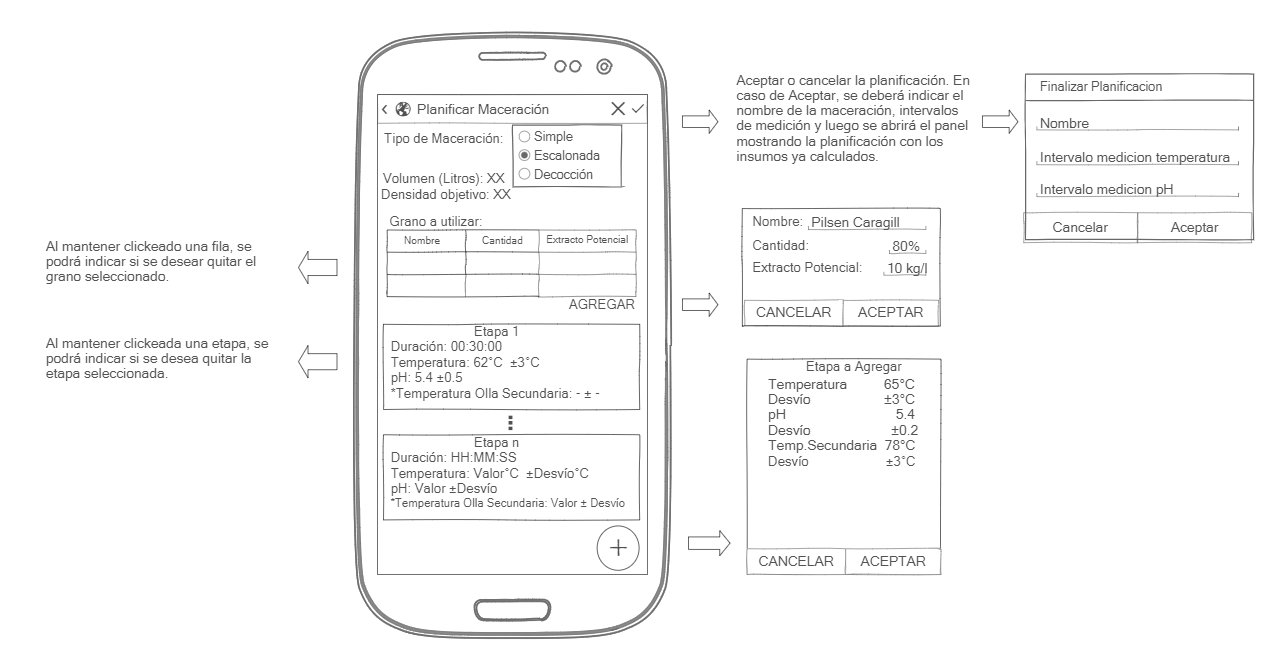
\includegraphics[scale=0.55, angle =90]{Anexo/MockUp/PlanningActivity.jpg}
        \captionof{figure}{Pantalla de planificación de maceración}
        \label{fig:MockUpPlanningActivity}
    \end{minipage}
    
    \begin{minipage}{0.95\textwidth}

        \centering
        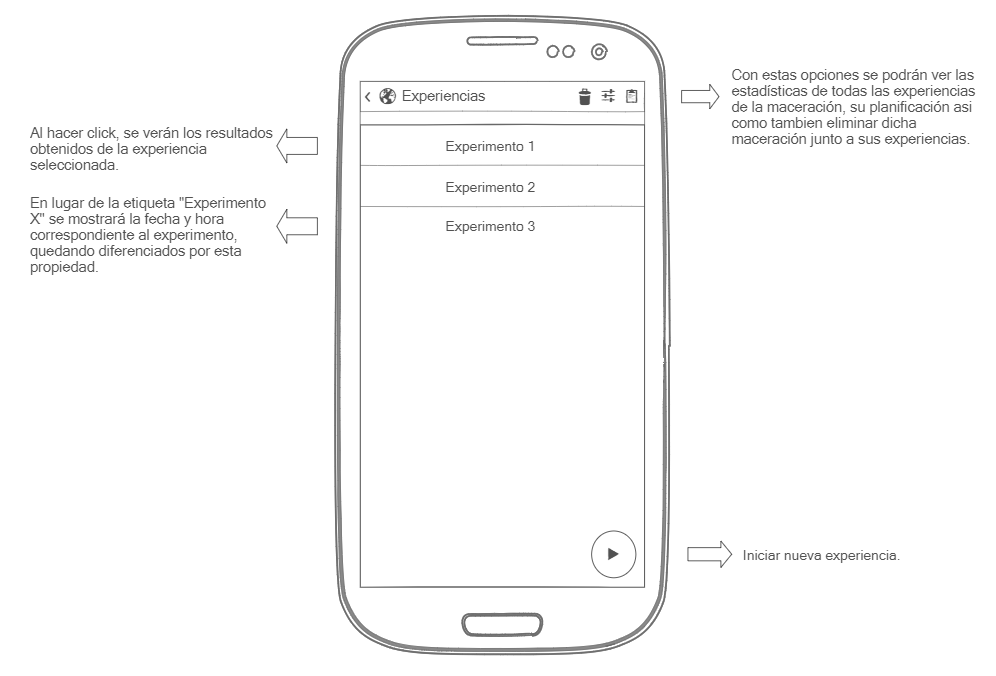
\includegraphics[scale=0.55]{Anexo/MockUp/ExperimentActivity.jpg}
        \captionof{figure}{Pantalla con lista de experimentos de una maceración}
        \label{fig:MockUpExperimentActivity}
    \end{minipage}
    
    \begin{minipage}{0.95\textwidth}

        \centering
        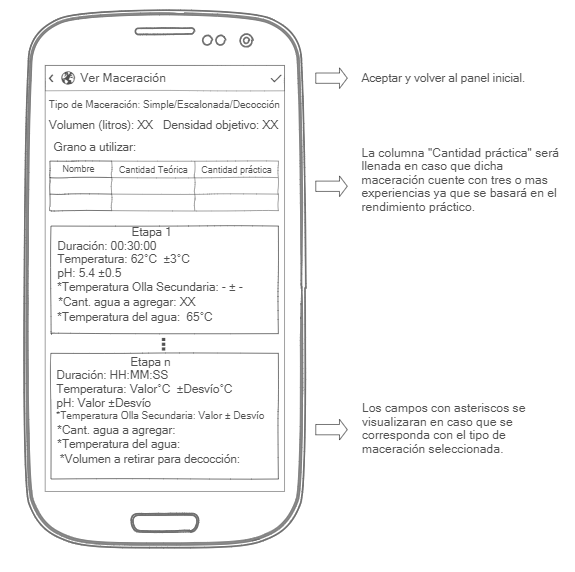
\includegraphics[scale=0.7]{Anexo/MockUp/InfoMash.jpg}
        \captionof{figure}{Pantalla con información de la maceración}
        \label{fig:MockUpInfoMash}
    \end{minipage}
    
    \begin{minipage}{0.95\textwidth}

        \centering
        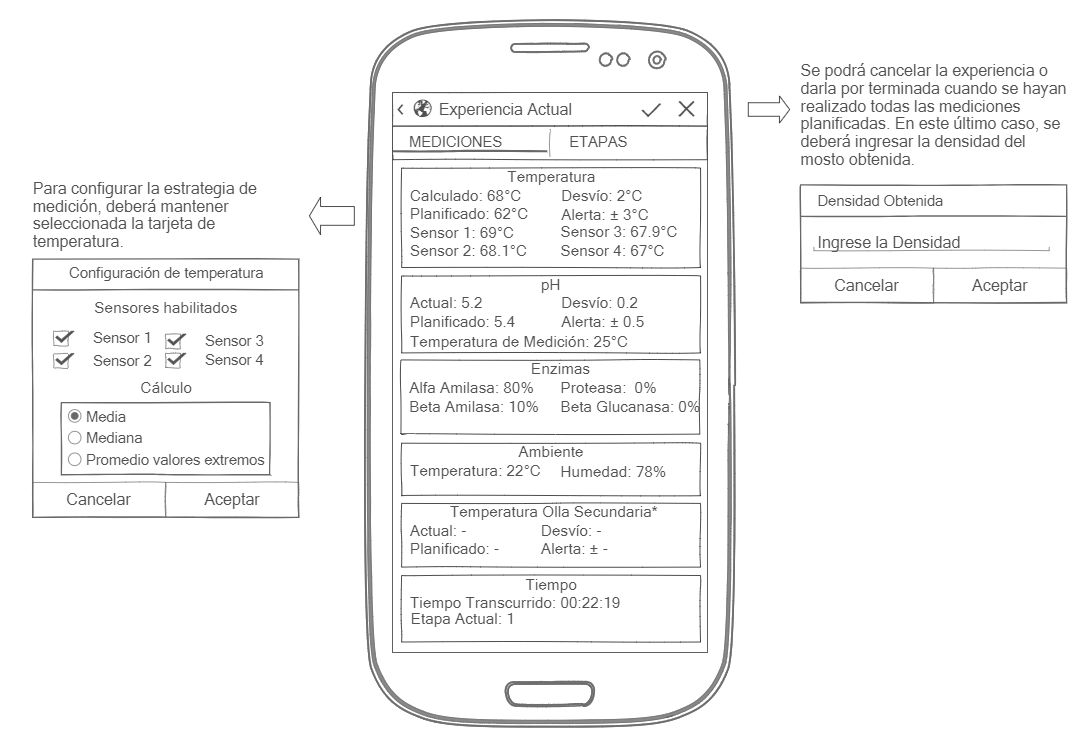
\includegraphics[scale=0.5]{Anexo/MockUp/CurrentExperience-MeasureFragment.jpg}
        \captionof{figure}{Pantalla de mediciones del experimento en ejecución}
        \label{fig:MockUpCurrentExperienceFragment}
    \end{minipage}
    
    \begin{minipage}{0.95\textwidth}

        \centering
        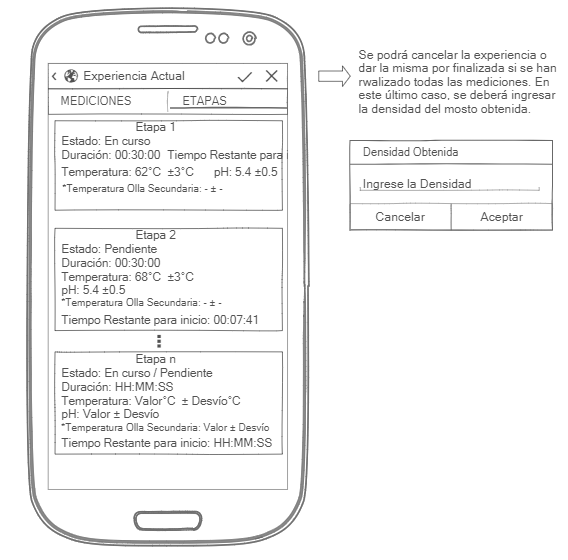
\includegraphics[scale=0.7]{Anexo/MockUp/CurrentExperience-StageFragment.jpg}
        \captionof{figure}{Pantalla con información de las etapas del experimento en ejecución}
        \label{fig:MockUpStageFragment}
    \end{minipage}
    
    \begin{minipage}{0.95\textwidth}

        \centering
        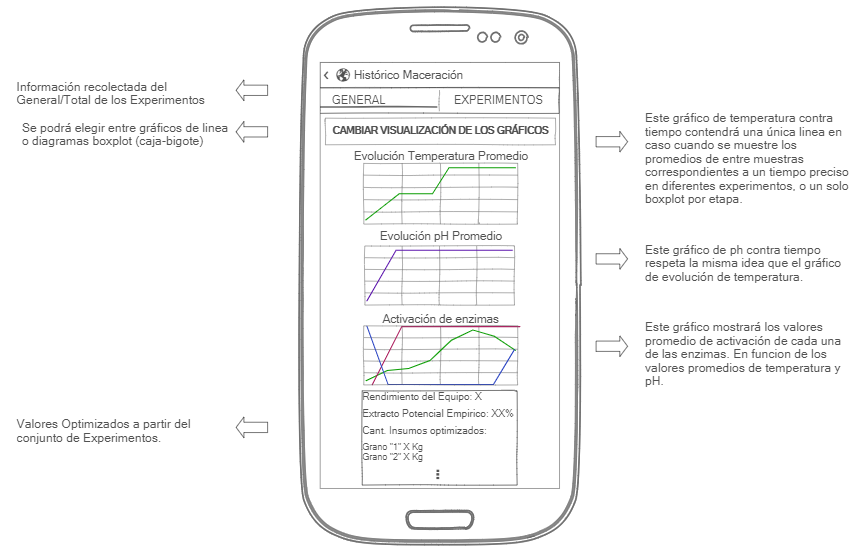
\includegraphics[scale=0.7]{Anexo/MockUp/MashExpHistoryActivity-GeneralFragment.jpg}
        \captionof{figure}{Pantalla con información estadística descriptiva de mediciones y de optimización de insumos y rendimiento}
        \label{fig:MockUpGeneralFragment}
    \end{minipage}
    
    \begin{minipage}{0.95\textwidth}

        \centering
        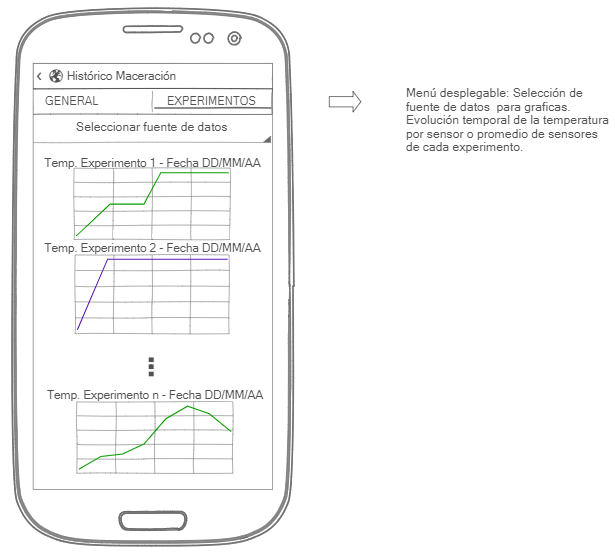
\includegraphics[scale=0.7]{Anexo/MockUp/MashExpHistoryActivity-ExperimentFragment.jpg}
        \captionof{figure}{Pantalla con información estadística descriptiva de mediciones de temperatura de cada experimento}
        \label{fig:MockUpExperimentFragment}
    \end{minipage}
    
   \begin{minipage}{0.95\textwidth}

        \centering
        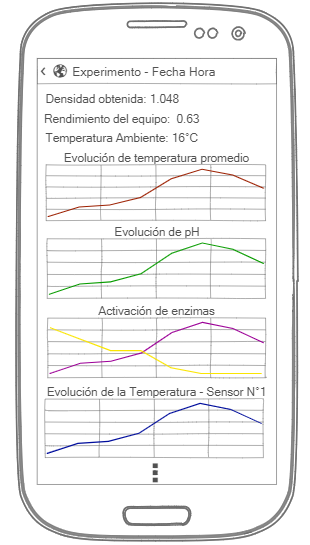
\includegraphics[scale=0.7]{Anexo/MockUp/DetailExperimentActivity.jpg}
        \captionof{figure}{Pantalla con información detalladas de los resultados de cada experimento}
        \label{fig:MockUpDetailExperimentActivity}
    \end{minipage}
    
%-------------------------- DIAGRAMAS DE CLASE --------------------------- 
    \begin{minipage}{0.95\textwidth}
    \chapter{Diagramas de clases}
    %\begin{figure}
        \centering
        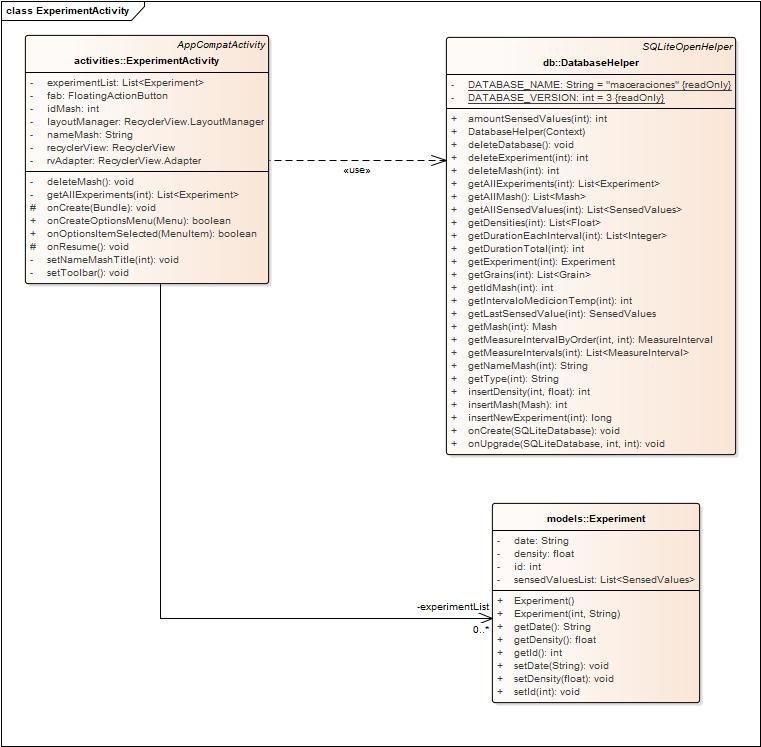
\includegraphics[scale=0.55, angle=90]{Anexo/DiagramasClase/ExperimentActivity.jpg}
        \captionof{figure}{Diagrama de clases de ExperimentActivity}
        \label{fig:DiagClaseExperimentActivity}
    %\end{figure}
    \end{minipage}
    
    %\begin{minipage}{0.95\textwidth}
            \begin{figure}
                \centering
                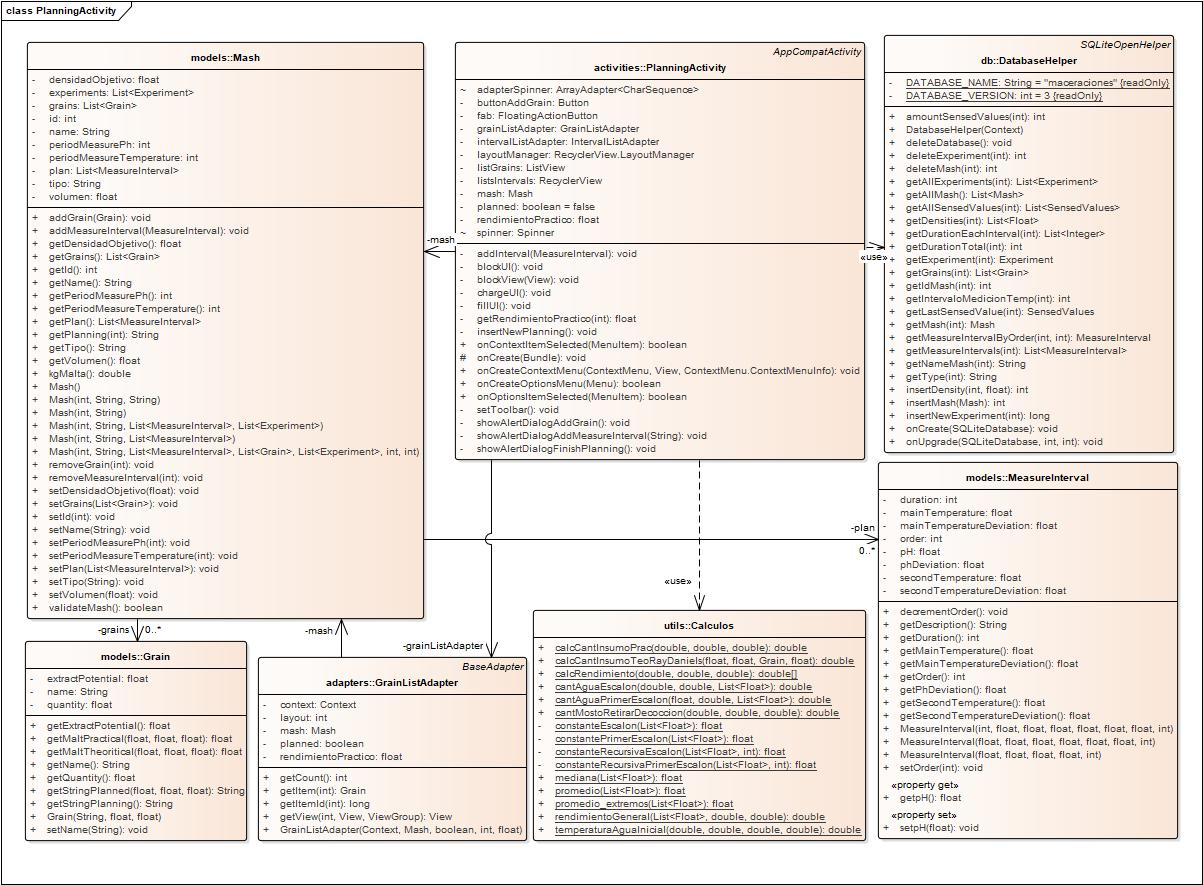
\includegraphics[scale=0.5, angle=90]{Anexo/DiagramasClase/PlanningActivity.jpg}
                \captionof{figure}{Diagrama de clases de PlanningActivity}
                \label{fig:DiagClasePlanningActivity}
            \end{figure}
    %\end{minipage}
    
    
    \begin{figure}
        %\section{Diagramas de clases}
        \centering
        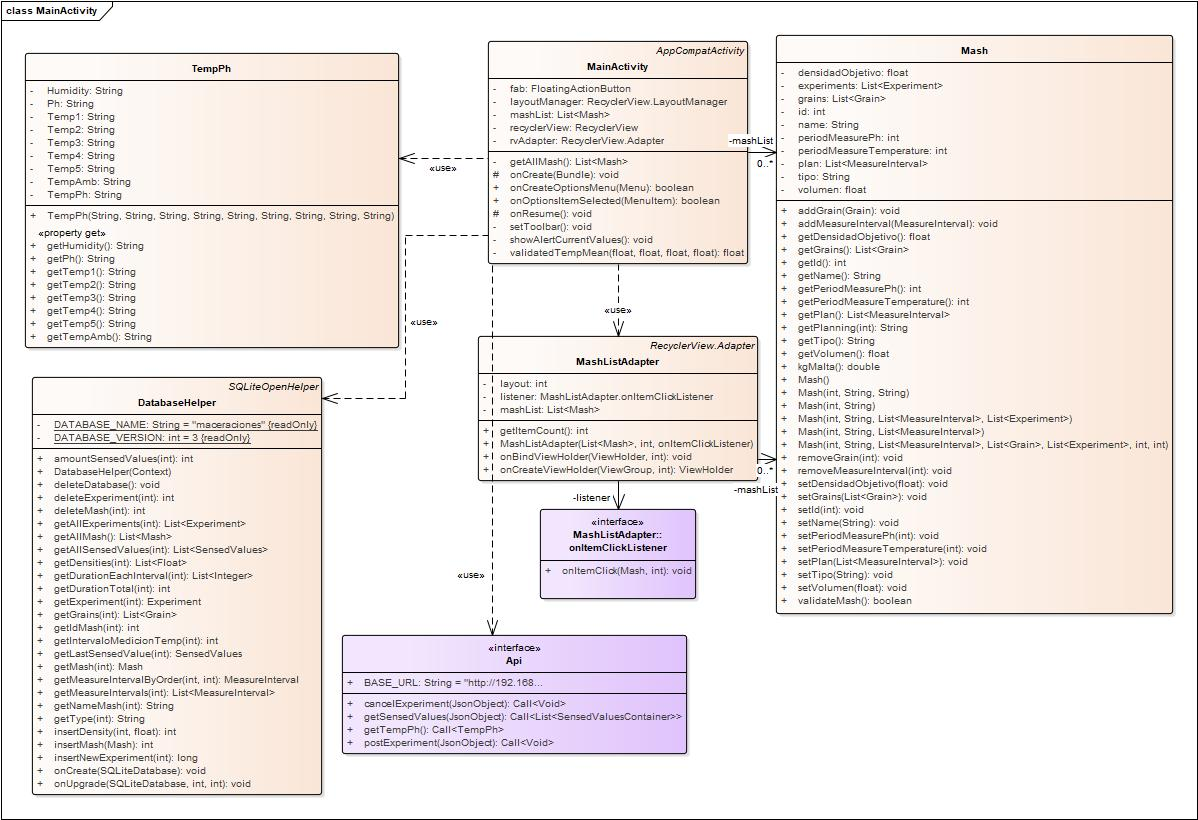
\includegraphics[scale=0.5, angle =90]{Anexo/DiagramasClase/MainActivity.jpg}
        \captionof{figure}{Diagrama de clases de MainActivity}
        \label{fig:DiagClaseMainActivity}
    \end{figure}
    
    
    %\begin{minipage}{0.95\textwidth}
    \begin{figure}
        \centering
        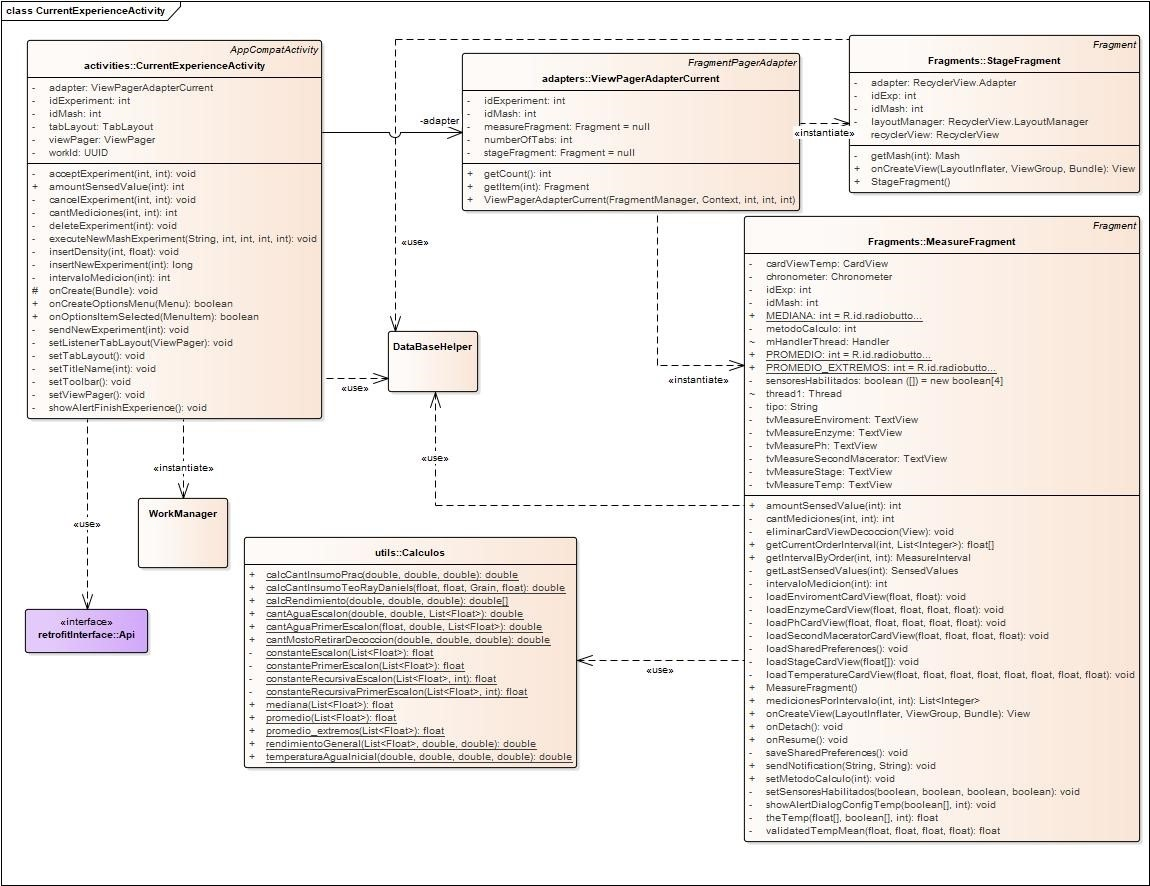
\includegraphics[scale=0.6, angle=90]{Anexo/DiagramasClase/CurrentExperienceActivity-P1.jpg}
        \captionof{figure}{Diagrama de clases de CurrentExperienceActivity - Parte 1}
        \label{fig:DiagClaseCurrentExperienceActivityP1}
    \end{figure}
    %\end{minipage}
    
    %\begin{minipage}{0.95\textwidth}
    \begin{figure}
        \centering
        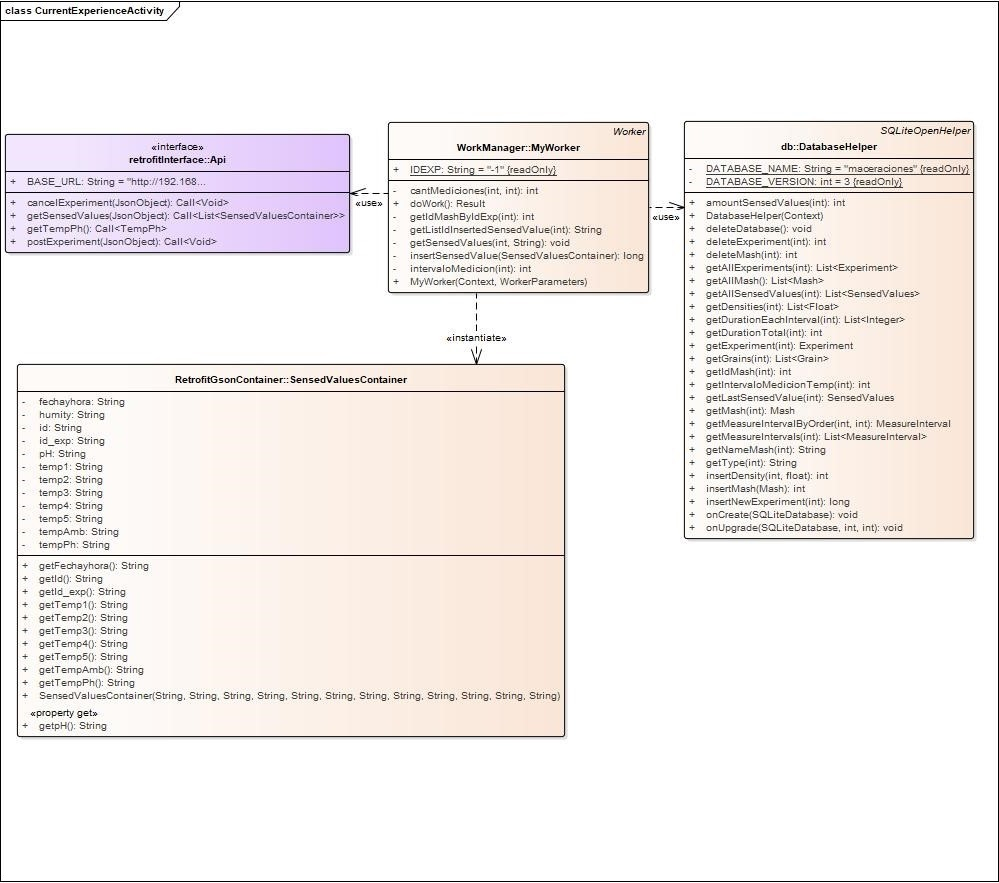
\includegraphics[scale=0.6, angle=90]{Anexo/DiagramasClase/CurrentExperienceActivity-P2.jpg}
        \captionof{figure}{Diagrama de clases de CurrentExperienceActivity - Parte 2}
        \label{fig:DiagClaseCurrentExperienceActivityP2}
    \end{figure}
    %\end{minipage}
    
    %\begin{minipage}{0.95\textwidth}
        \begin{figure}
        \centering
        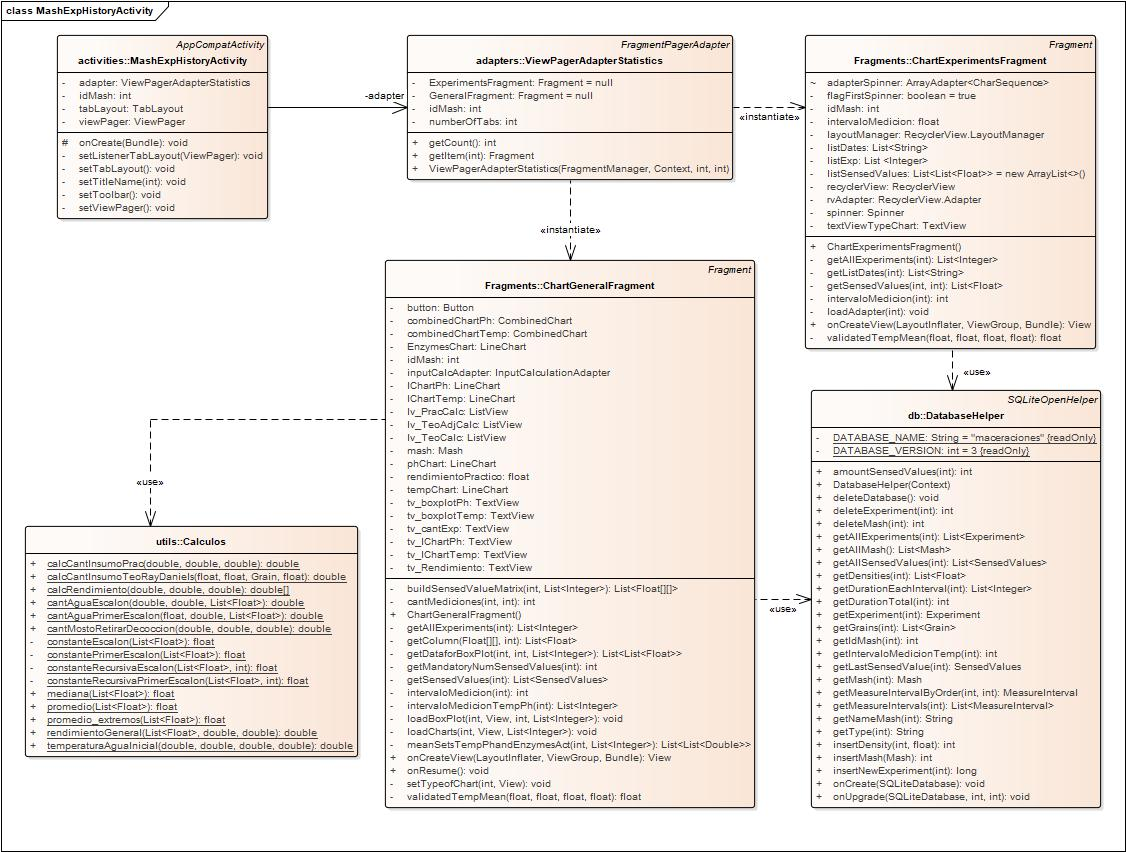
\includegraphics[scale=0.5, angle=90]{Anexo/DiagramasClase/MashExpHistoryActivity.jpg}
        \captionof{figure}{Diagrama de clases de MashExpHistoryActivity}
        \label{fig:DiagClaseMashExpHistoryActivity}
        \end{figure}
    %\end{minipage}
    
    %\begin{minipage}{0.95\textwidth}
        \begin{figure}
        \centering
        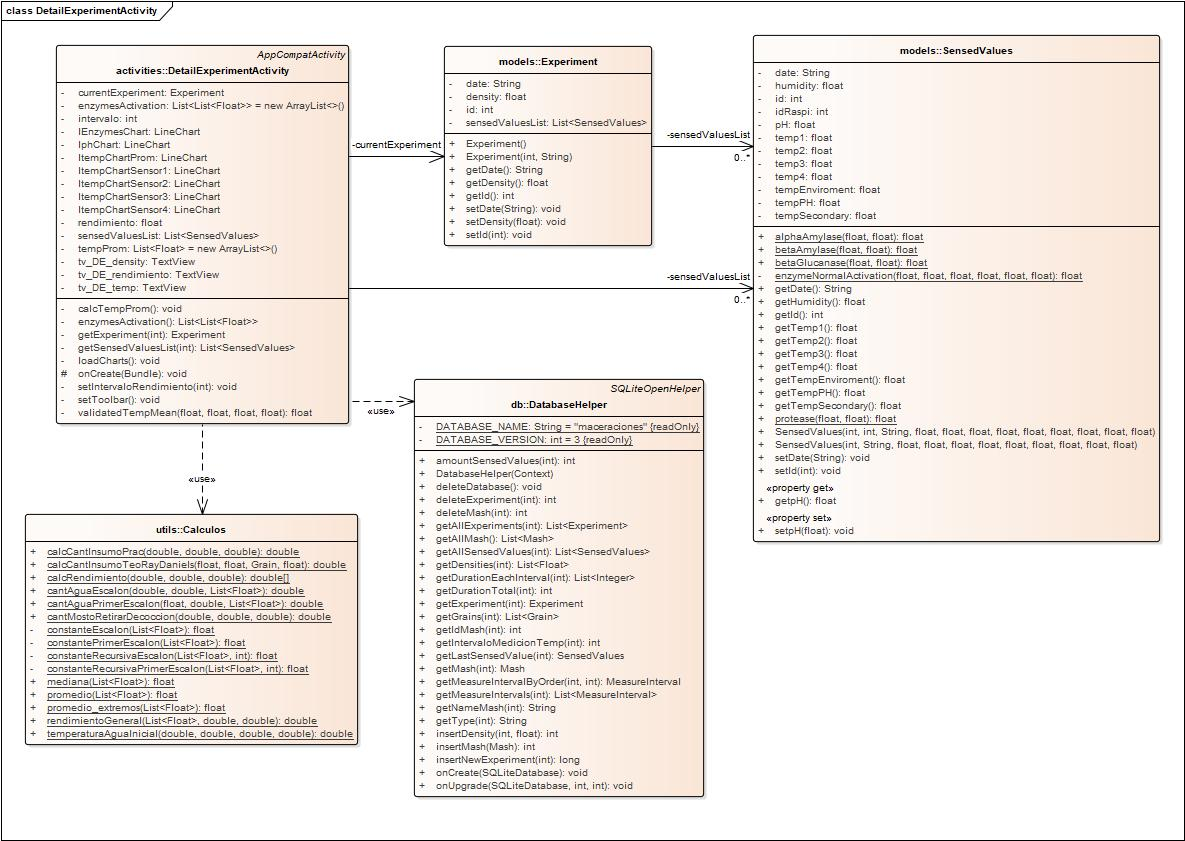
\includegraphics[scale=0.5, angle=90]{Anexo/DiagramasClase/DetailExperimentActivity.jpg}
        \captionof{figure}{Diagrama de clases de DetailExperimentActivity}
        \label{fig:DiagClaseDetailExperimentActivity}
        \end{figure}
    %\end{minipage}
    
    \begin{figure}
        \centering
        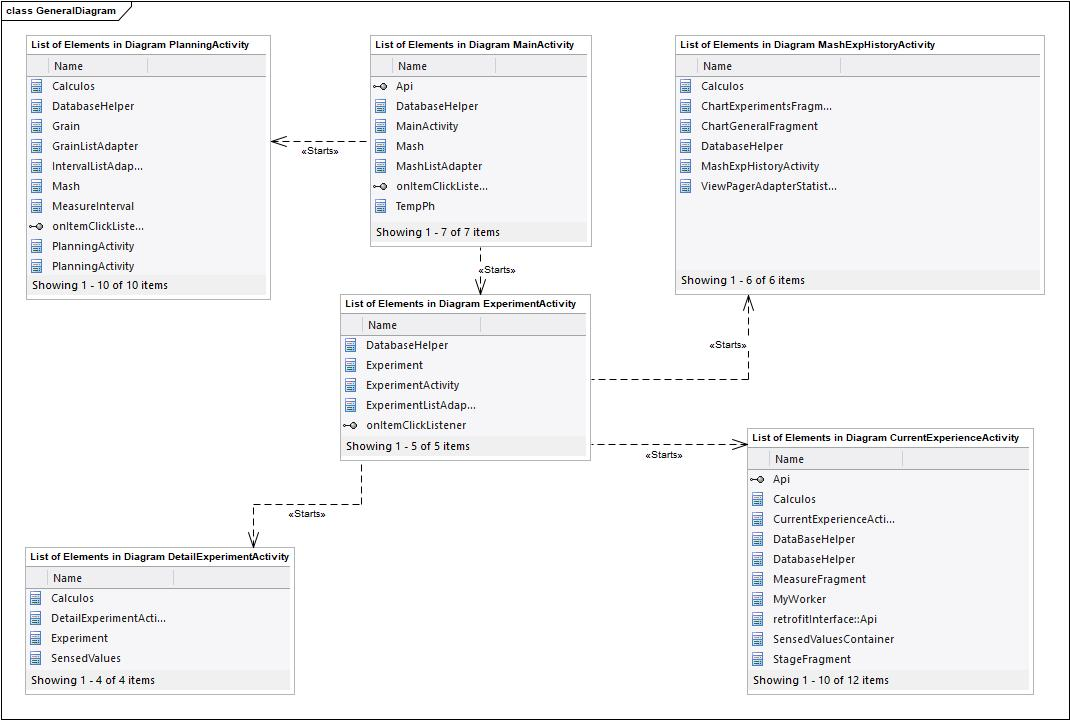
\includegraphics[scale=0.5, angle=90]{Anexo/DiagramasClase/GeneralDiagram.jpg}
        \captionof{figure}{Diagrama General de la Aplicación}
        \label{fig:DiagGeneral}
        \end{figure}
    
    %\begin{minipage}{0.95\textwidth}
    %\begin{minipage}{0.95\textwidth}
    \chapter{Fotografías de prueba de campo}
    \label{AnexoFotografias}
        \centering
        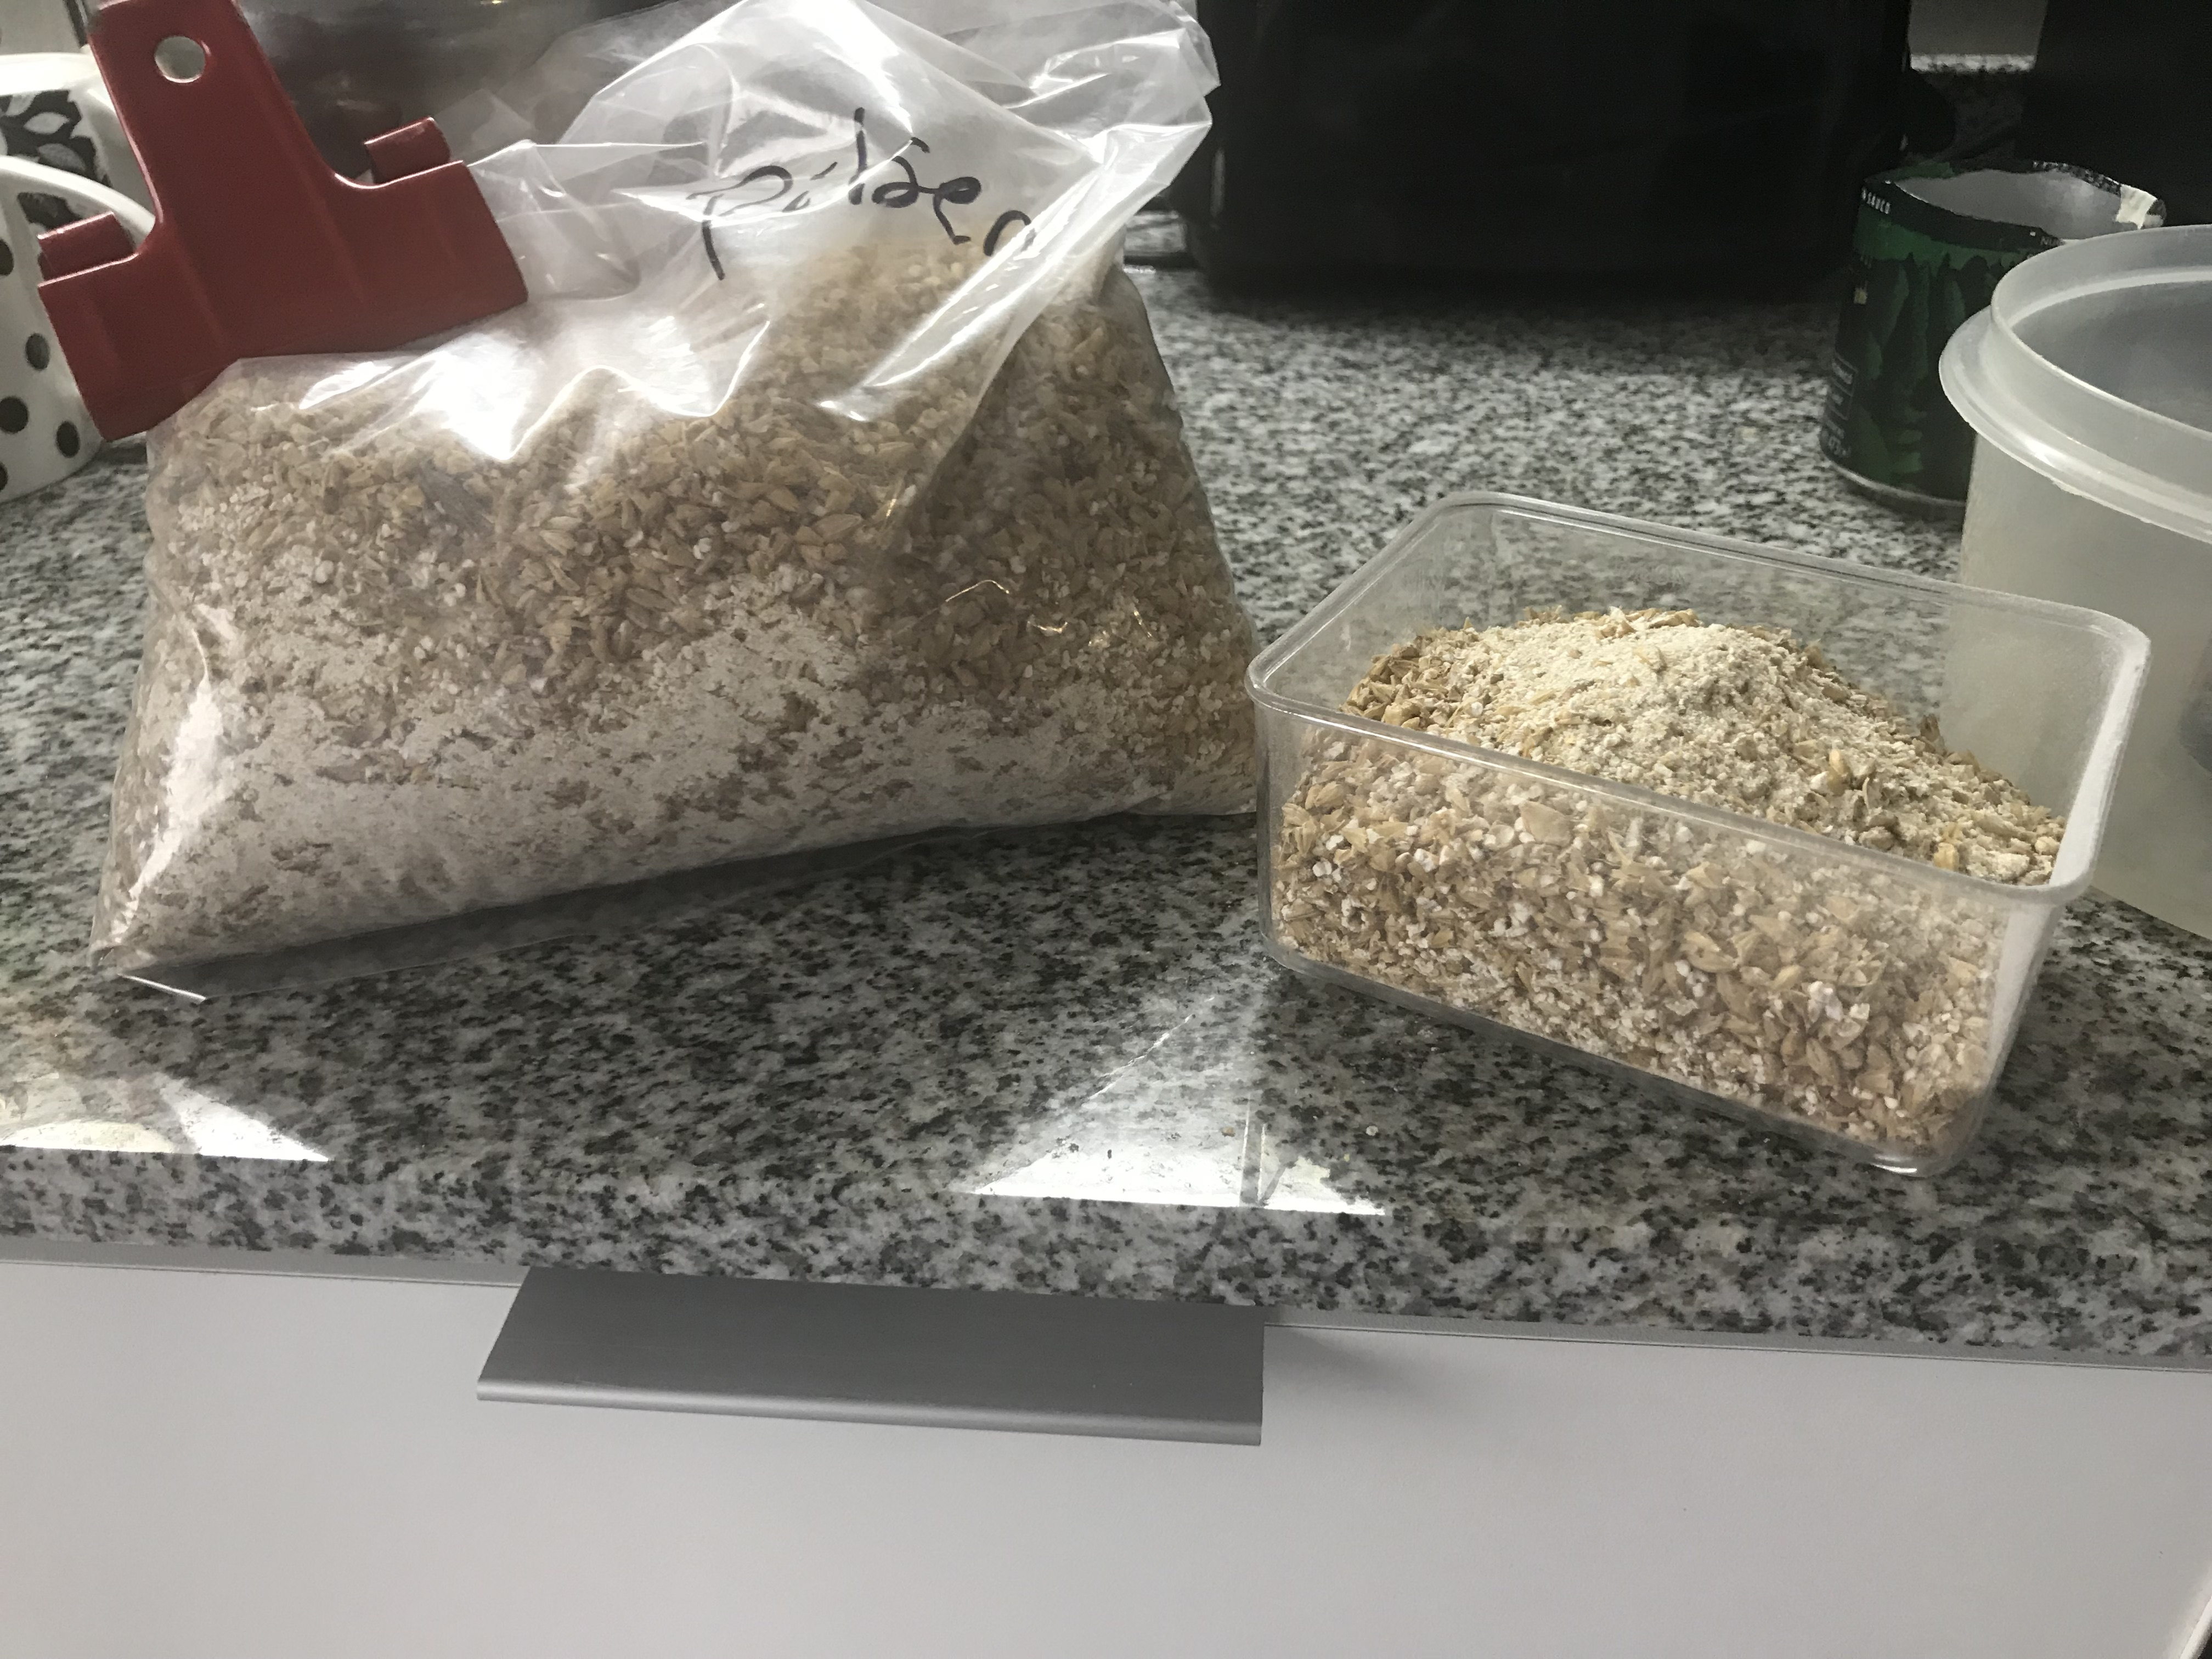
\includegraphics[scale=0.10]{Anexo/FotosExperimentos/P1.jpg}
        \captionof{figure}{Insumos}
        \label{fig:InsumosMalta}
    %\end{minipage}
        
    \begin{figure}
        \centering
        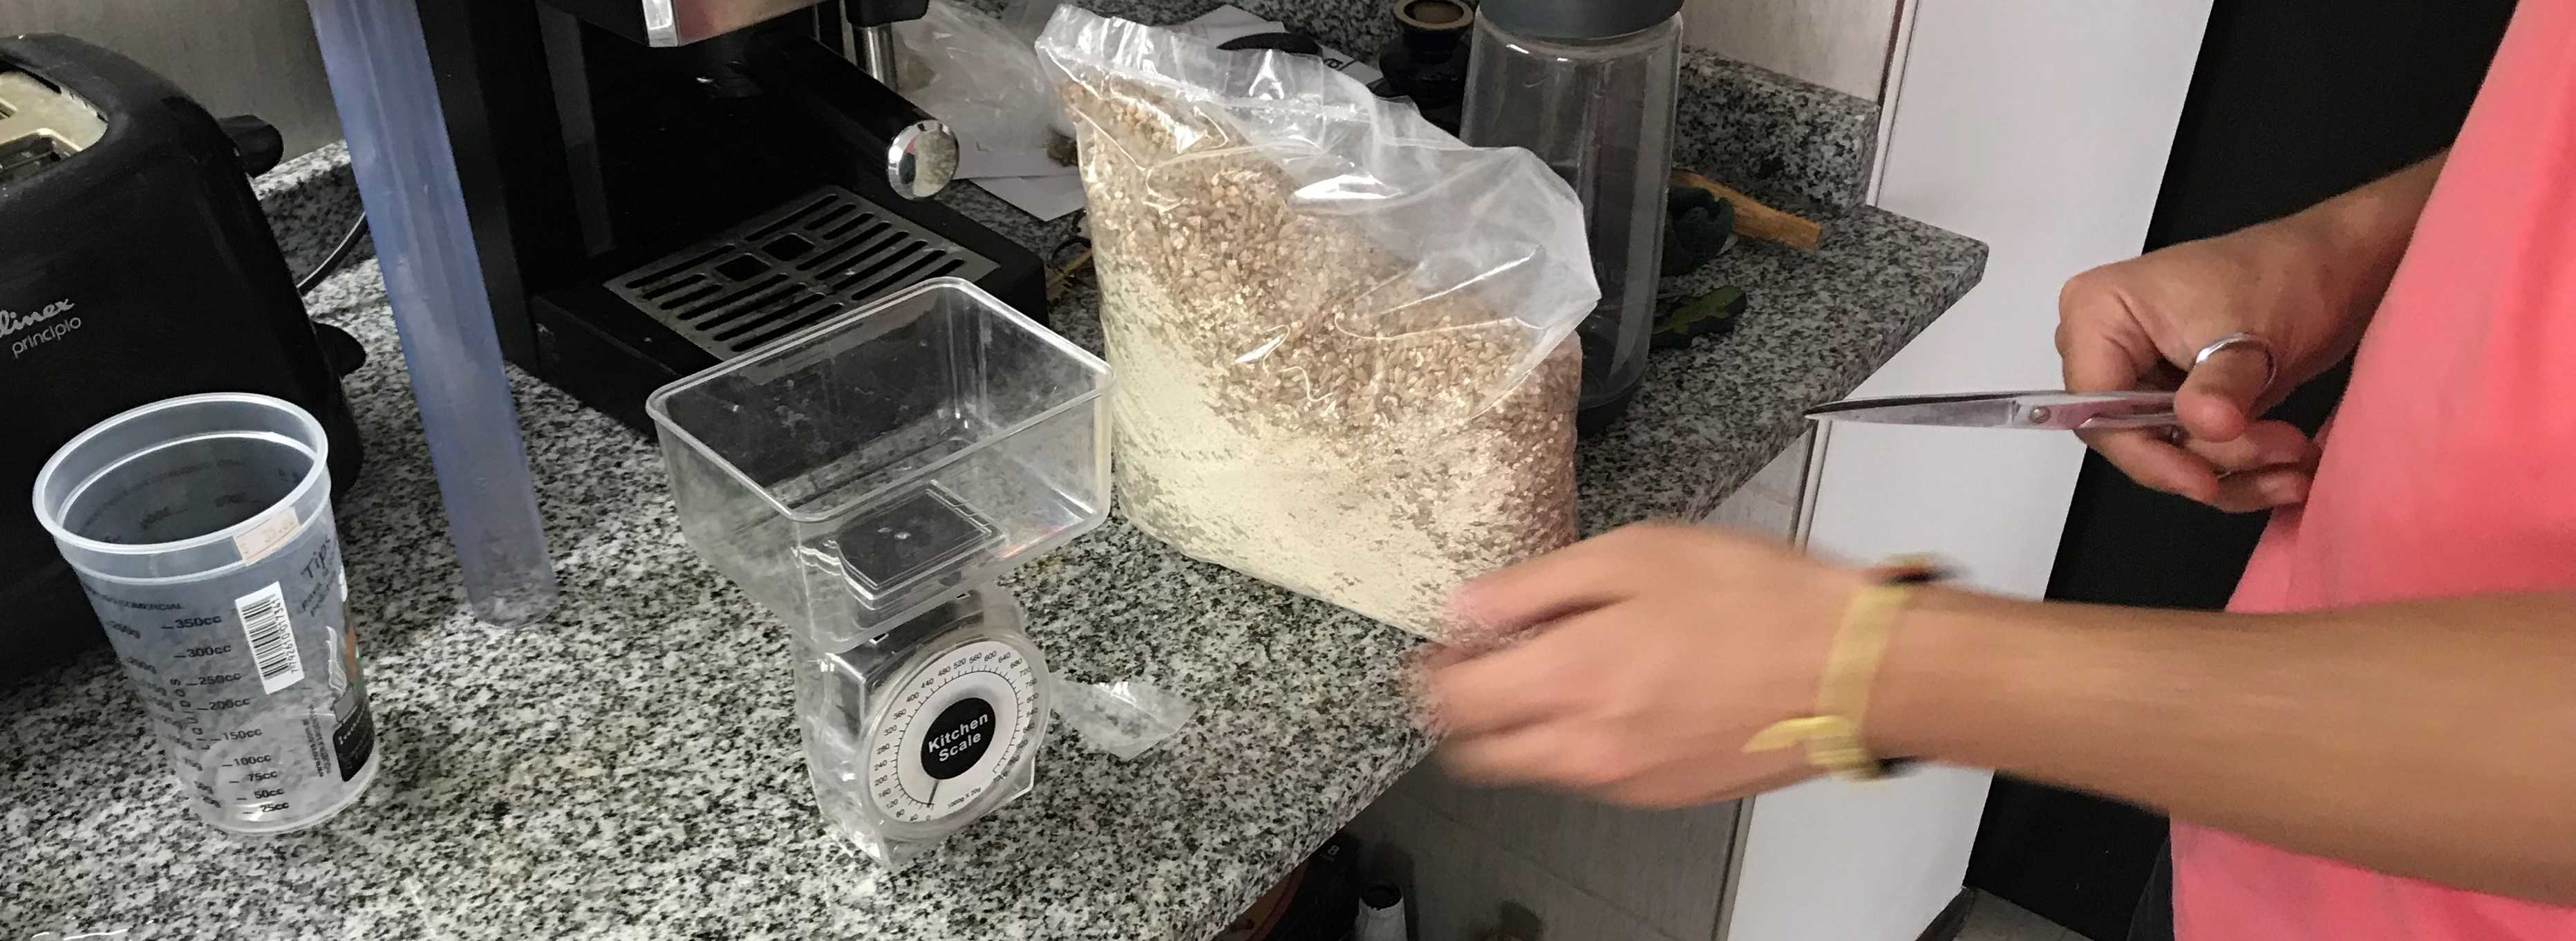
\includegraphics[scale=0.10]{Anexo/FotosExperimentos/P2.jpg}
        \captionof{figure}{Fragmentación de insumos}
        \label{fig:FragInsumos}
    \end{figure}
        
    \begin{figure}
        \centering
        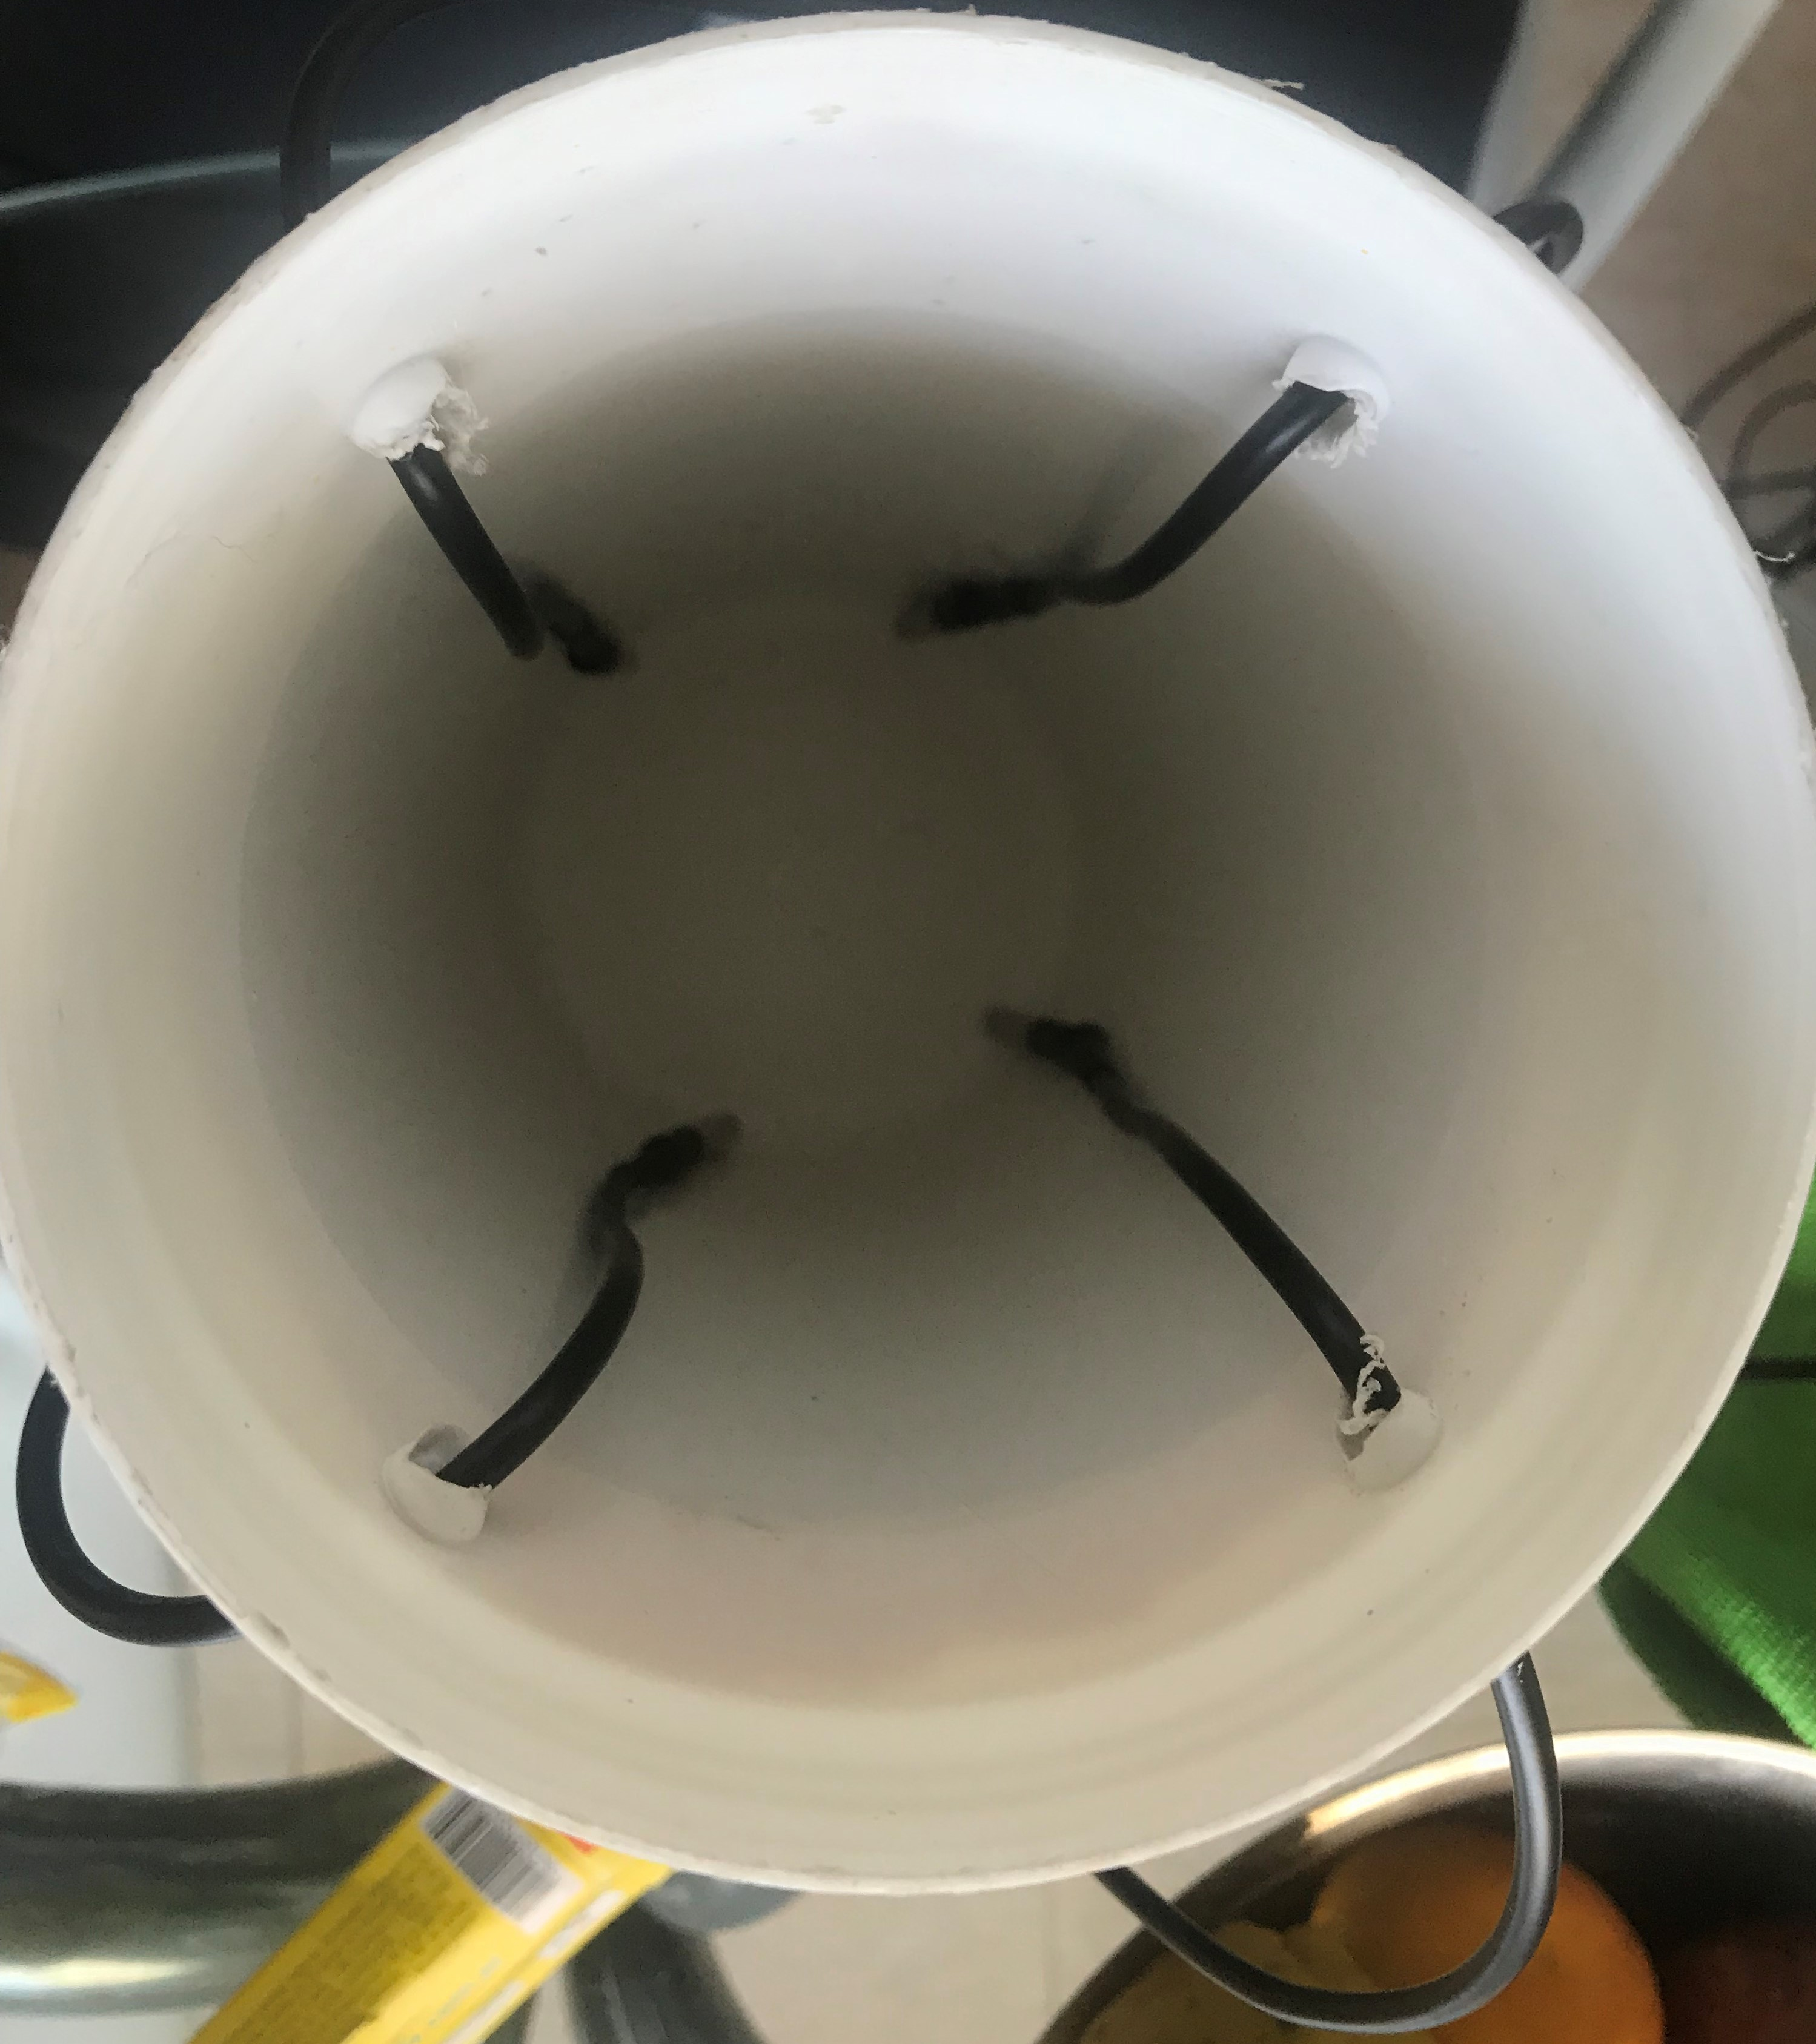
\includegraphics[scale=0.10]{Anexo/FotosExperimentos/P3.jpg}
        \captionof{figure}{Interior del termo}
        \label{fig:ConstrucMacerador}
    \end{figure}
    
    \begin{figure}
        \centering
        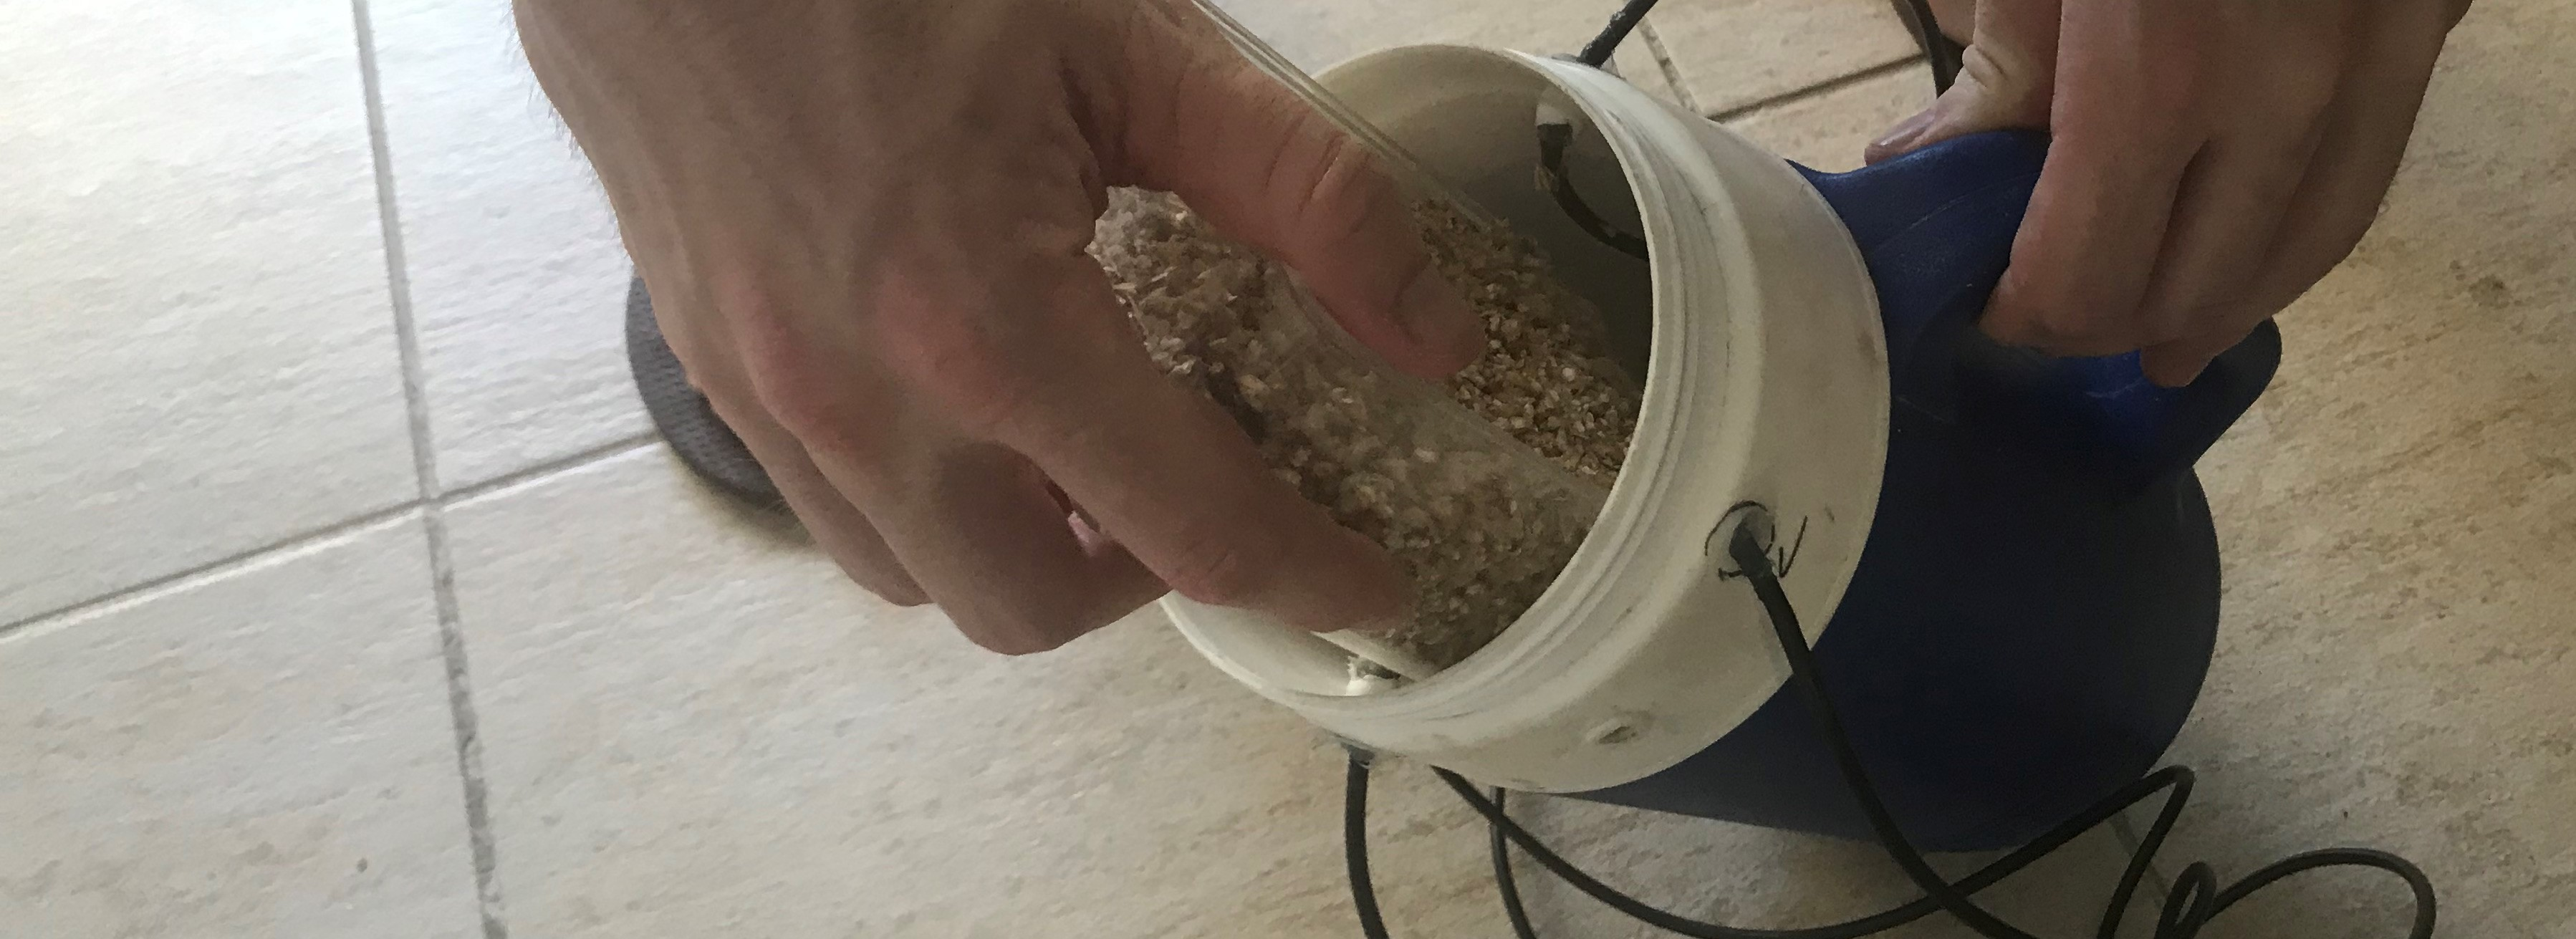
\includegraphics[scale=0.10]{Anexo/FotosExperimentos/P4.jpg}
        \captionof{figure}{Incorporación de insumos al macerador}
        \label{fig:IncorpInsumos}
    \end{figure}
    
    \begin{figure}
        \centering
        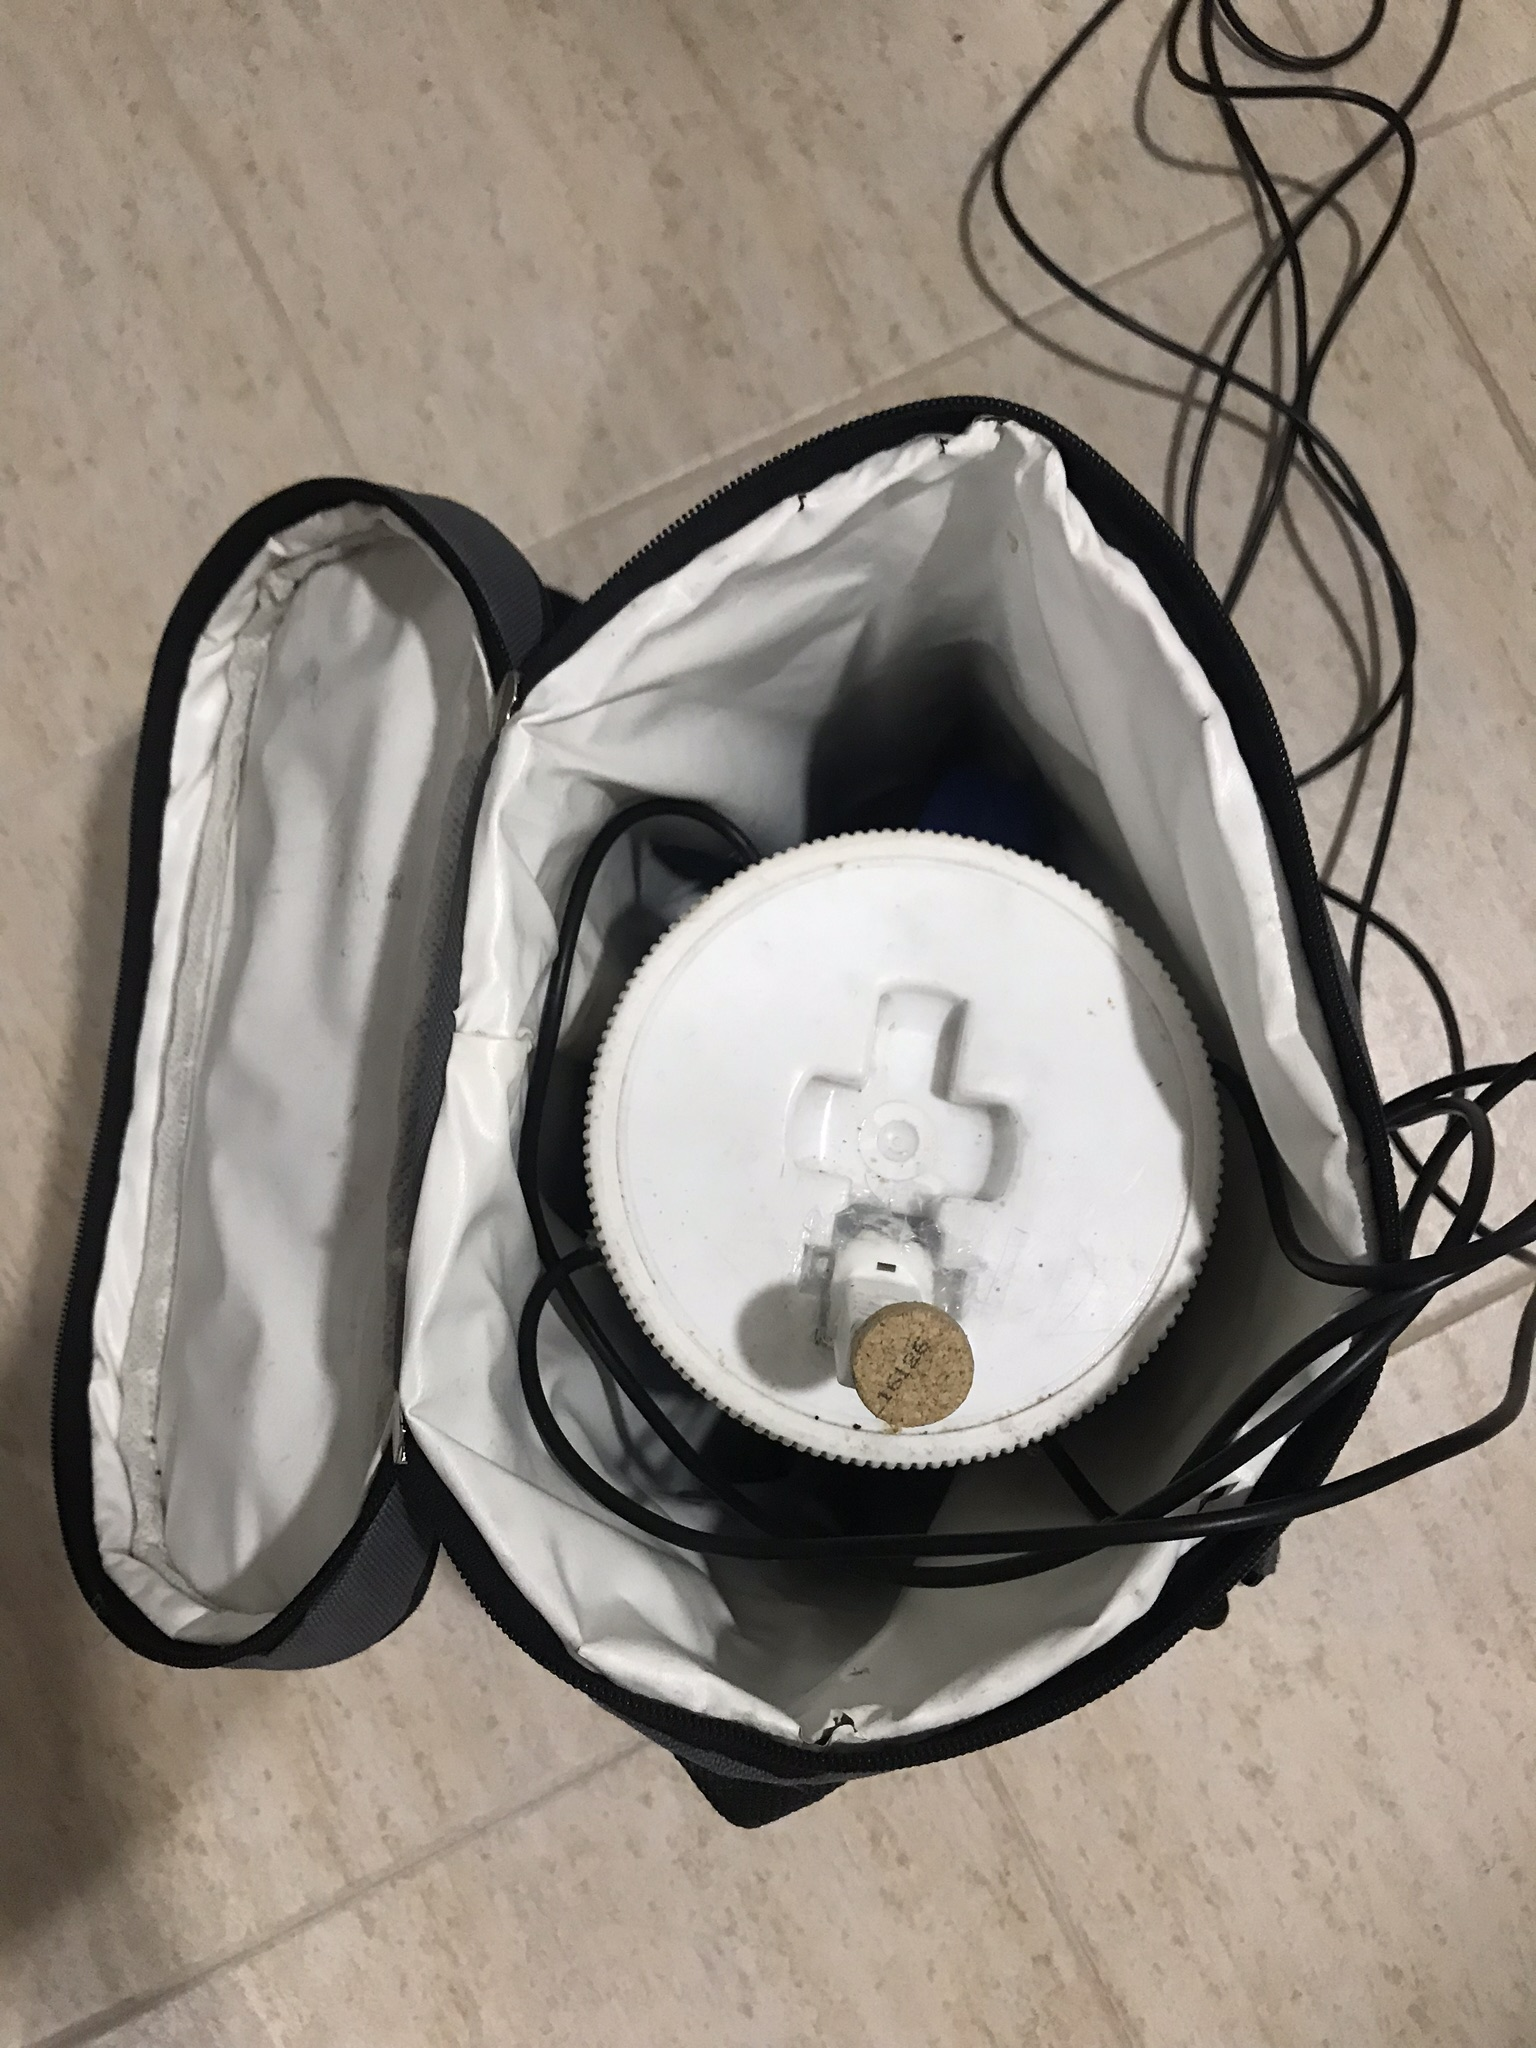
\includegraphics[scale=0.10]{Anexo/FotosExperimentos/P5.jpeg}
        \captionof{figure}{Aislamiento térmico}
        \label{fig:ConstrucAislamTerm}
    \end{figure}
    
    \begin{figure}
        \centering
        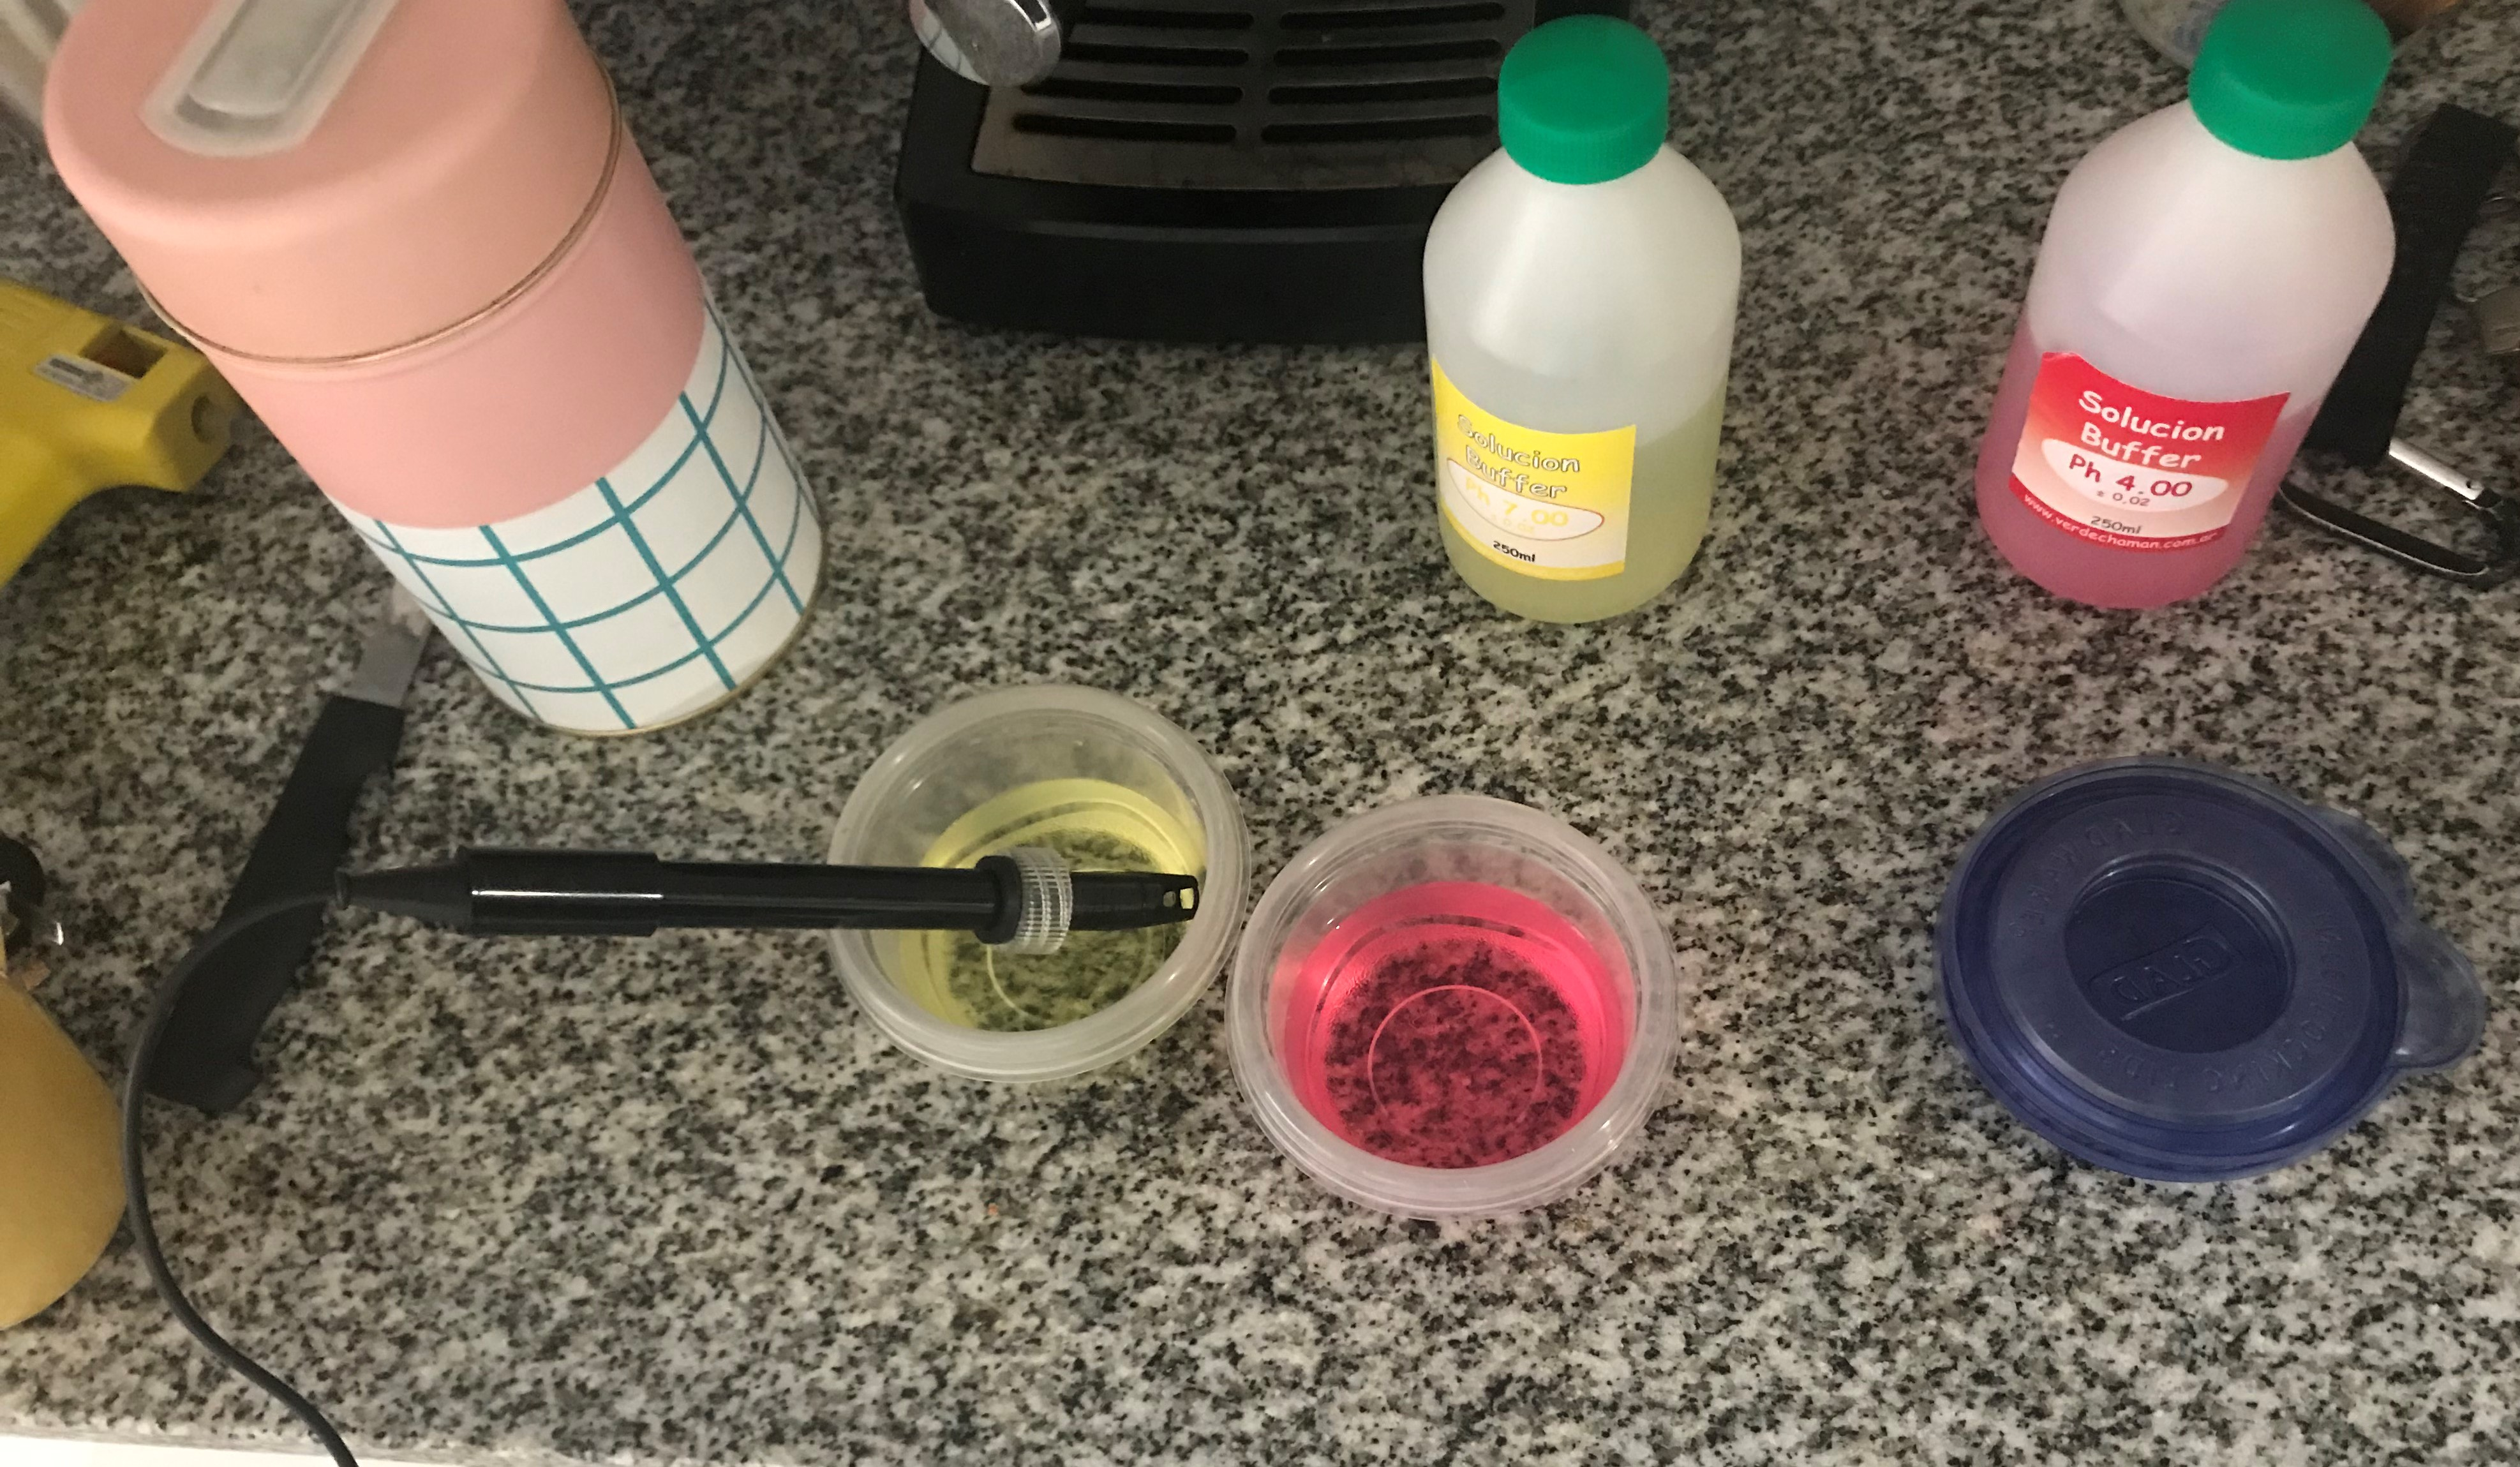
\includegraphics[scale=0.10]{Anexo/FotosExperimentos/P6.jpg}
        \captionof{figure}{Calibración del sensor de pH}
        \label{fig:CalibrPhimetro}
    \end{figure}
        
    \begin{figure}
        \centering
        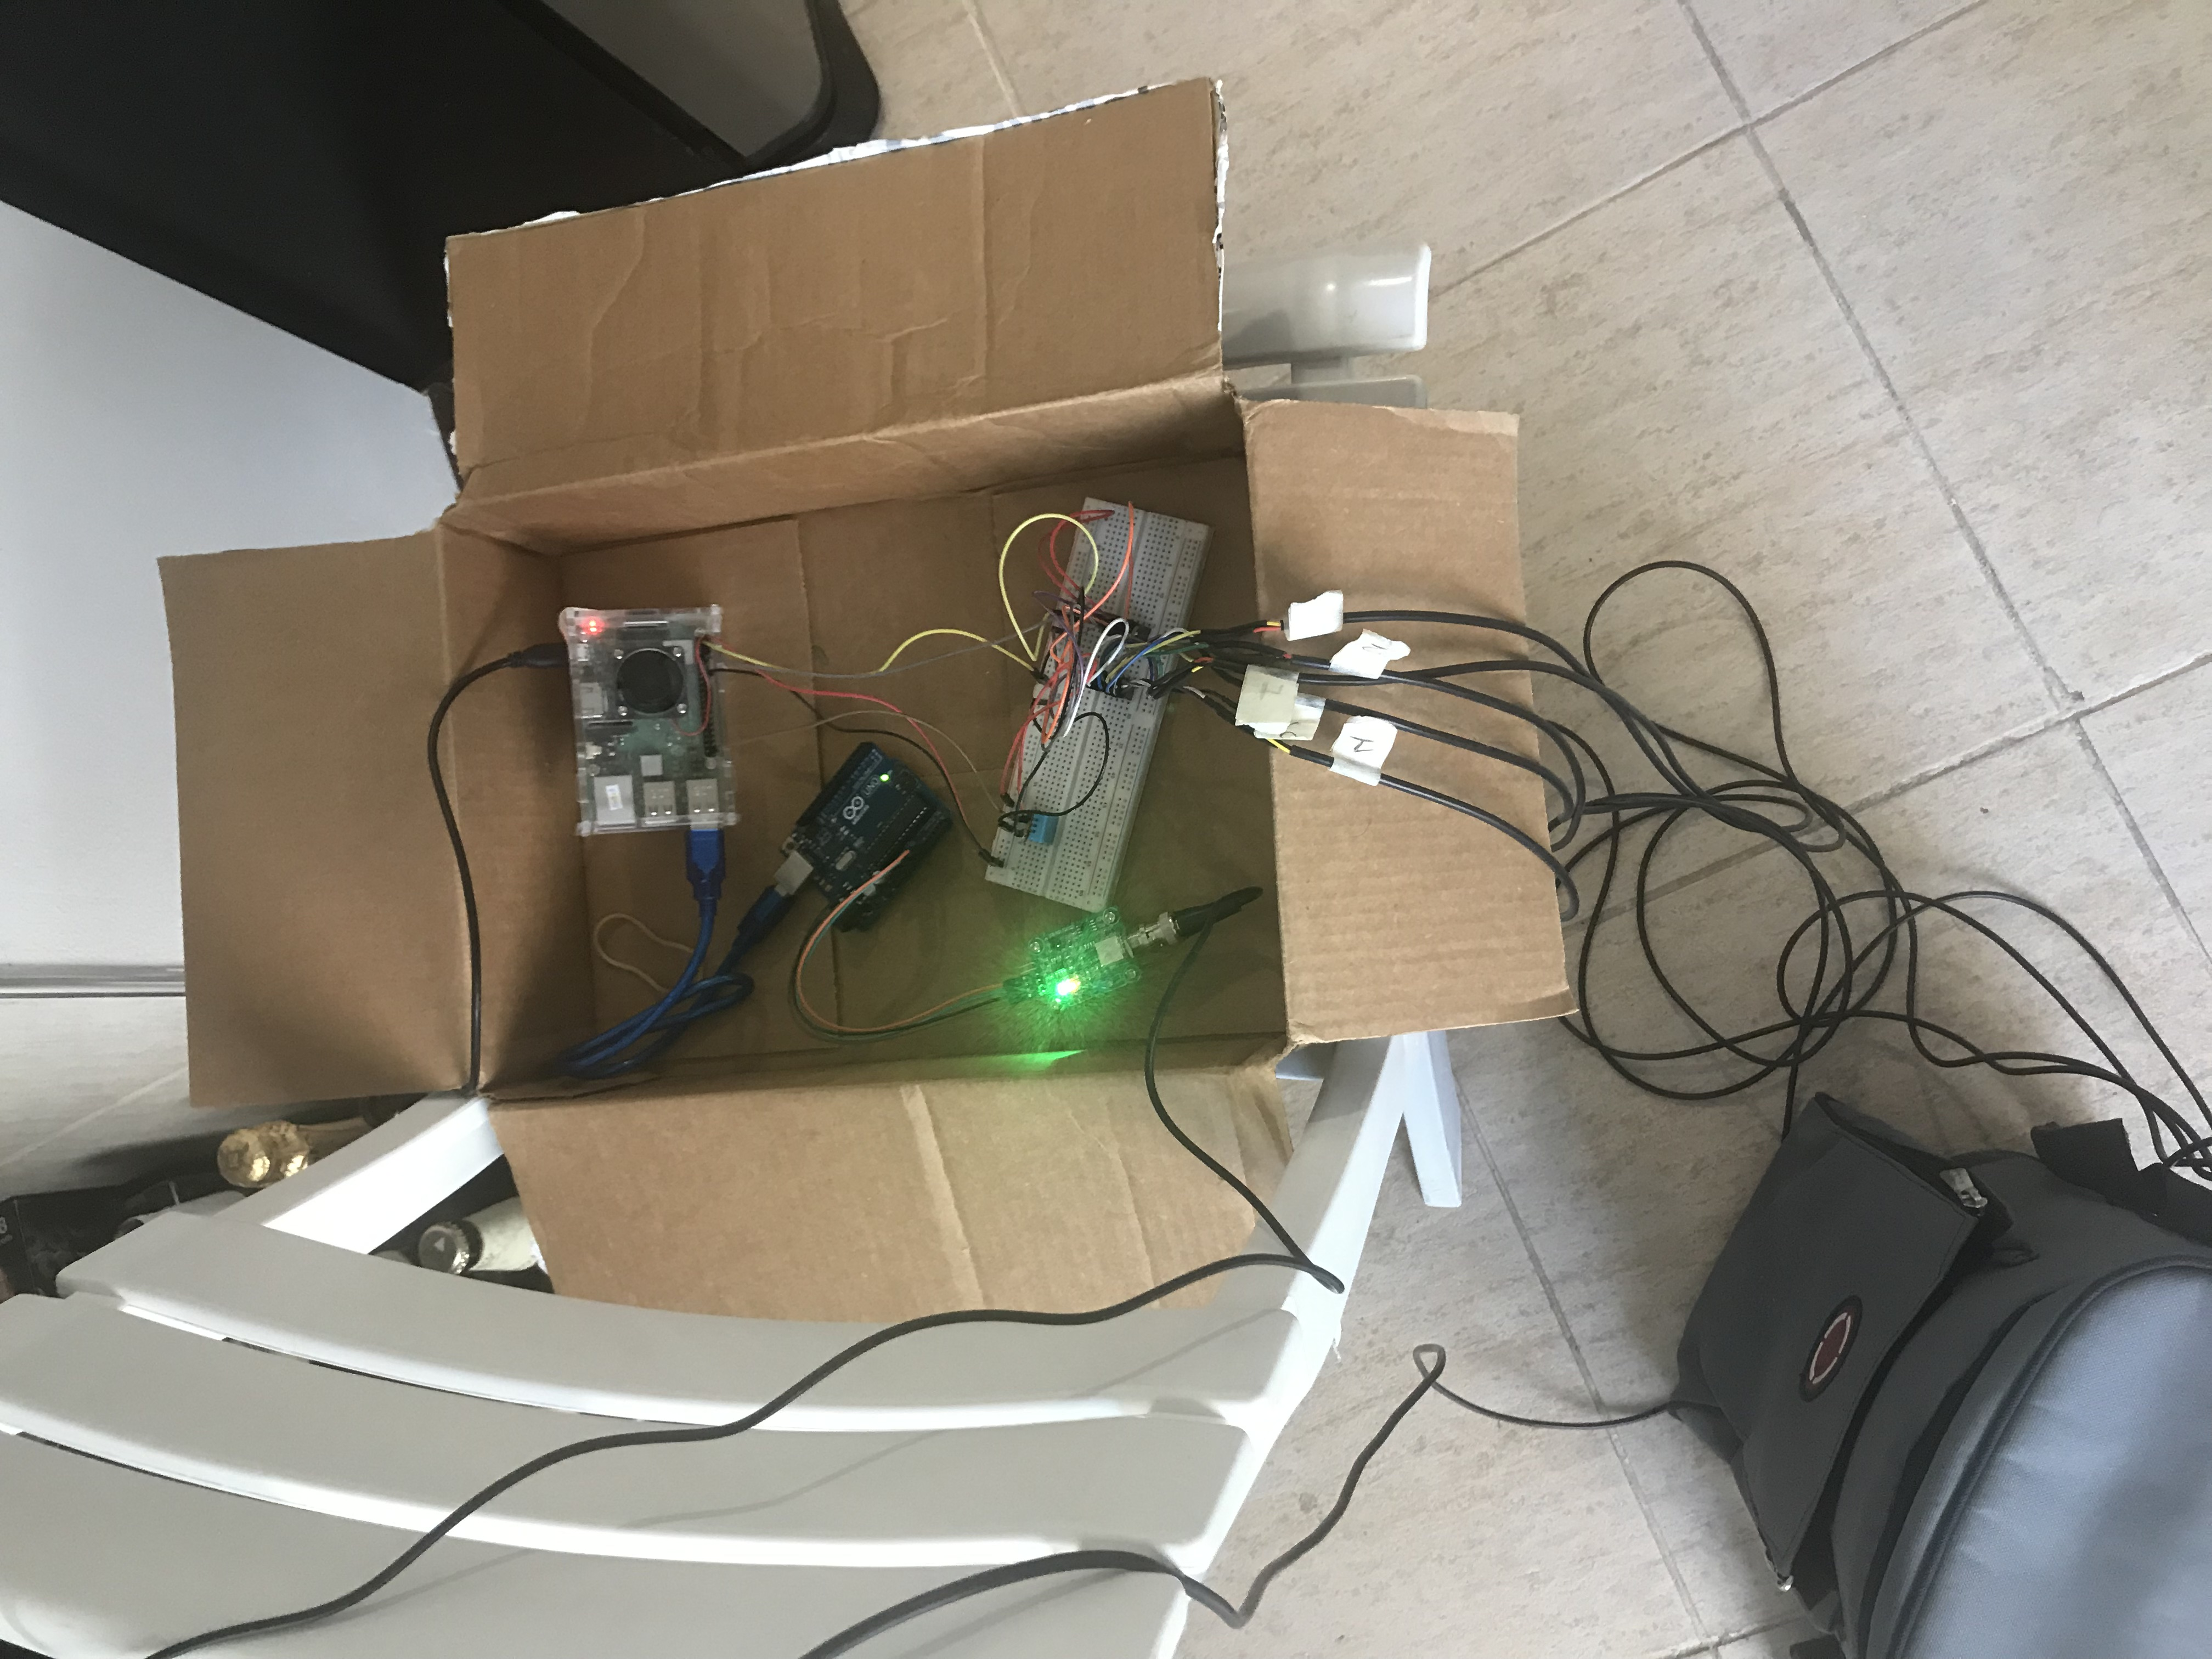
\includegraphics[scale=0.1]{Anexo/FotosExperimentos/P7.jpg}
        \captionof{figure}{Montaje del sistema}
        \label{fig:MontajeSist}
    \end{figure}
    
    \begin{figure}
        \centering
        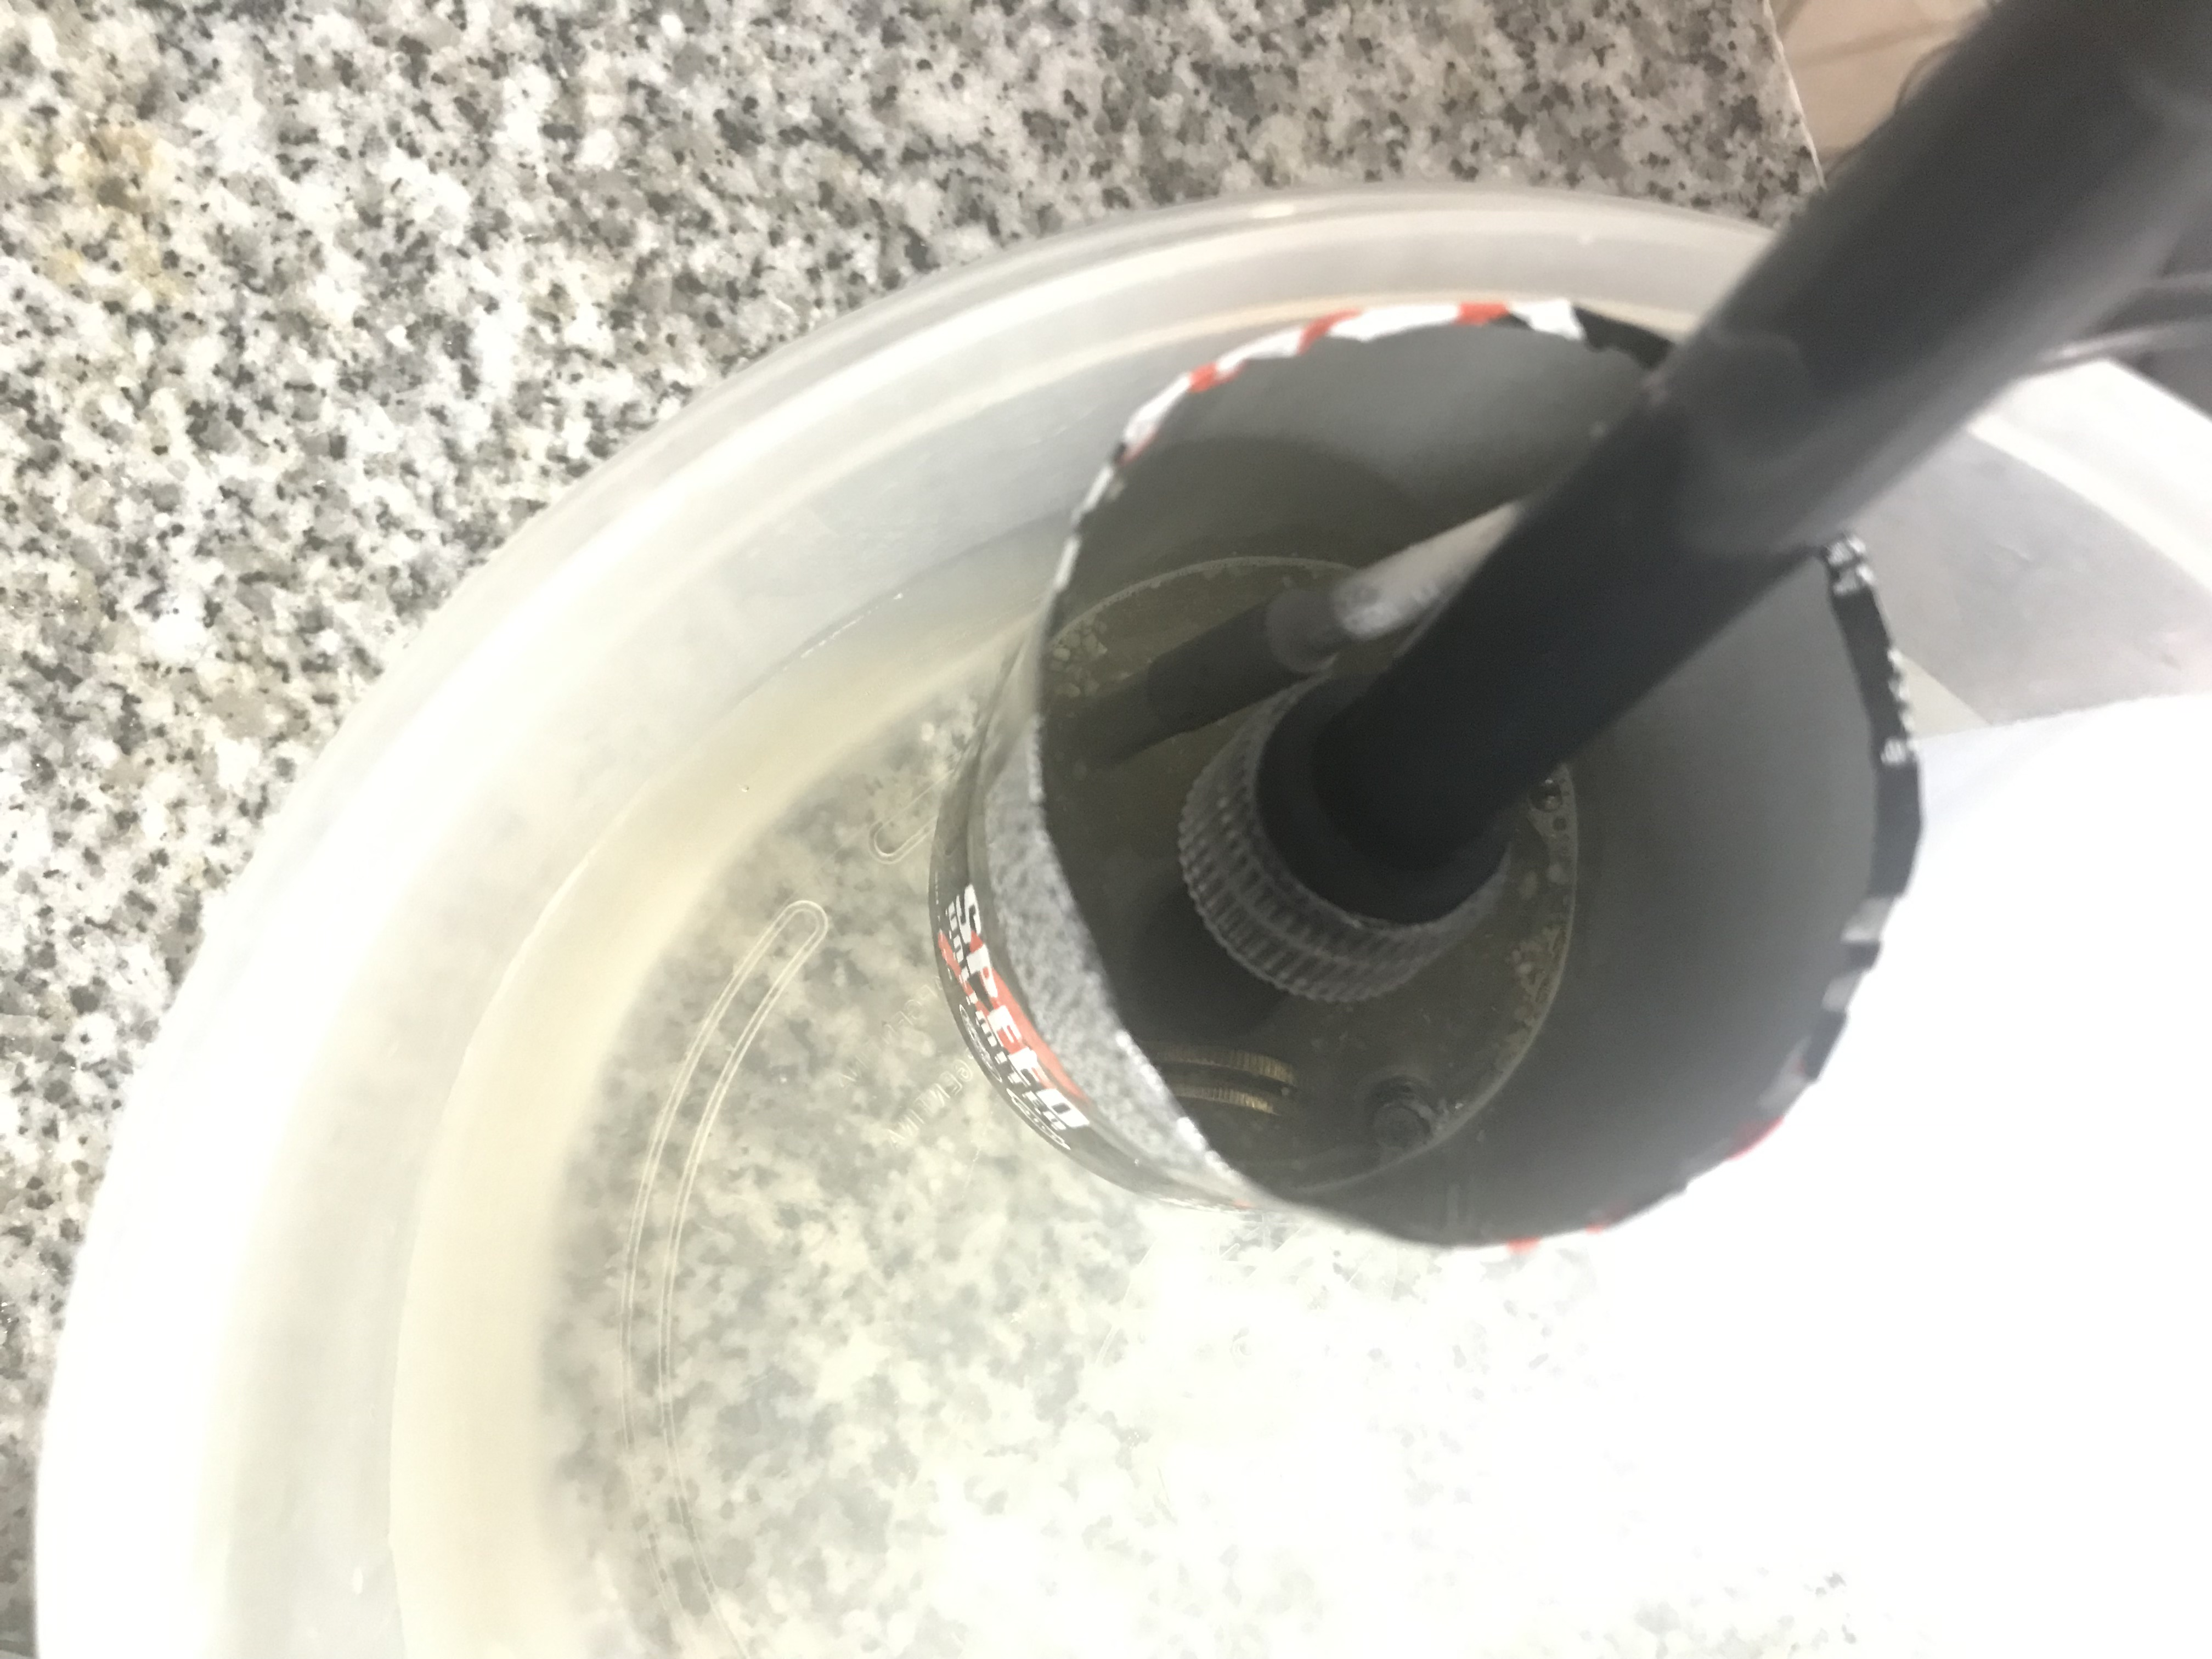
\includegraphics[scale=0.1]{Anexo/FotosExperimentos/P8.jpg}
        \captionof{figure}{Refrigerador de muestras}
        \label{fig:MedicPH}
    \end{figure}
        
    %\end{minipage}
    \begin{minipage}{0.95\textwidth}
    \chapter{Casos de prueba}
    \label{CasosPrueba}
    \begin{center}
    \begin{tabularx}{\textwidth}{ | p{2cm} | X | X | X |}
        \hline
        \multicolumn{4}{|c|}{\textbf{Caso de Prueba: Monitorear variables - CP001}} \\
        \hline
        \multicolumn{4}{|l|}{\textbf{Actor Caso de Prueba:} Productor de Cerveza} \\
        \hline
        \multicolumn{4}{|l|}{\textbf{Propósito}} \\
        \hline
        \multicolumn{4}{|p{0.95\linewidth}|}{Verificar la correcta funcionalidad del dialogo que proporciona los datos siendo recolectados por los sensores de la estación de recolección de datos. Verificar que se despliegan en pantalla los datos antes mencionados} \\
        \hline
        \multicolumn{4}{|l|}{\textbf{Descripción de las acciones para las pruebas}} \\
        \hline
        \textbf{\#} & Acciones & Salida Esperada & Salida Obtenida \\
        \hline
        01 & Abrir el panel mediante el botón destinado a ello presente en la pantalla principal & Se abre el panel y se despliegan los datos esperados. & El panel se abrió correctamente y se mostraron luego los datos esperados. \\
        \hline
        \multicolumn{4}{|c|}{\textbf{Resultados Obtenidos}} \\
        \hline
        \multicolumn{4}{|l|}{\textbf{Resultado:} Aprobado} \\
        \hline
        \multicolumn{4}{|l|}{\textbf{Evidencia: \url{https://shorturl.me/BauGZ} }} \\
        \hline
     \end{tabularx}
    \label{CP001}
    \end{center}
    %\end{minipage}
    
    %\begin{minipage}{0.95\textwidth}
    \begin{center}
    \begin{tabularx}{\textwidth}{ | p{2cm} | X | X | X |}
        \hline
        \multicolumn{4}{|c|}{\textbf{Caso de Prueba: Planificar una maceración - CP002 (parte 1)}} \\
        \hline
        \multicolumn{4}{|l|}{\textbf{Actor Caso de Prueba:} Productor de Cerveza} \\
        \hline
        \multicolumn{4}{|l|}{\textbf{Propósito}} \\
        \hline
        \multicolumn{4}{|p{0.95\linewidth}|}{Verificar la correcta apertura y funcionalidad de la pantalla destinada para la carga y creación de una nueva maceración.} \\
        \hline
        \multicolumn{4}{|l|}{\textbf{Descripción de las acciones para las pruebas}} \\
        \hline
        \textbf{\#} & Acciones & Salida Esperada & Salida Obtenida \\
        \hline
        01 & Apertura de la pantalla mediante el botón destinado a ello presente en la pantalla principal & Se abre la pantalla con el formulario. & La pantalla se abrió correctamente desplegando en ella el formulario a rellenar. \\
        \hline
        02 & Agregar grano (formulario incompleto), apertura del diálogo y relleno incompleto del formulario & Se abre el diálogo con el formulario. No se agrega el grano y despliega un mensaje de error. & Se abrió el diálogo con el formulario. No se agregó el grano y desplegó un mensaje de error:"No se pudo insertar el grano porque faltaron completar campos". \\
        \hline
        
        \end{tabularx}
        \label{CP002-p1}
        \end{center}
        \end{minipage}
        
        
        \begin{minipage}{0.95\textwidth}
        \begin{center}
        \begin{tabularx}{\textwidth}{ | p{2cm} | X | X | X |}
        \hline
        \multicolumn{4}{|c|}{\textbf{Caso de Prueba: Planificar una maceración - CP002 (parte 2)}} \\
        \hline
        03 & Agregar grano (formulario completo), apertura del diálogo y relleno completo del formulario, luego se agrega el mismo pudiendo ver los datos del mismo en el formulario principal & Se abre el diálogo con el formulario, se rellena el mismo y luego es agregado el grano a la lista de granos. & Se abrió el diálogo con el formulario. El grano fue agregado a la lista. \\
        \hline
        04 & Eliminar grano, se abre el menú con la opción de eliminación luego de realizar una presión larga de un grano de la lista. Luego de seleccionada la eliminación en el menú, el mismo es retirado de la lista. & Se abre el menú, se selecciona eliminar y el mismo es removido de la lista. & Se abrió el menú, se seleccionó eliminar y el mismo fue removido de la lista de granos. \\
        \hline
        05 & Agregar nuevo intervalo de medición (formulario incompleto), luego de presionado el botón para este fin se abre un diálogo y se rellena de forma incompleta el formulario.  & No se agrega el intervalo a la lista de intervalos y se despliega un mensaje de error. & Se abrió el diálogo con el formulario. El intervalo no fue agregado a la lista y se desplegó un mensaje de error: "No se pudo insertar el intervalo porque faltaron completar campos" \\
        \hline
        06 & Agregar nuevo intervalo de medición (formulario completo), luego de presionado el botón para este fin se abre un diálogo y se rellena de forma completa el formulario presente en el mismo. & Se abre el diálogo con el formulario y luego es agregado el intervalo a la lista de intervalos. & Se abrió el diálogo con el formulario. El intervalo fue agregado a la lista.\\
        \hline
        07 & Finalizar carga de maceración (formulario principal, grano y/o intervalos no agregados). & Se presiona el botón de confirmación se despliega un error. & Se desplegó un mensaje de error por cada tipo de campo incompleto.\\
        \hline
        \end{tabularx}
        \label{CP002-p2}
        \end{center}
        \end{minipage}
        
        \begin{minipage}{0.95\textwidth}
        \begin{center}
        \begin{tabularx}{\textwidth}{ | p{2cm} | X | X | X |}
        \hline
        \multicolumn{4}{|c|}{\textbf{Caso de Prueba: Planificar una maceración - CP002 (parte 3)}} \\
        \hline
        08 & Finalizar carga de maceración (formulario principal completo, grano e intervalos agregados, formulario de finalización incompleto), luego de presionado el botón para este fin se despliega un dialogo con un formulario final, se rellena el formulario de forma incompleta. & Se presiona el botón de confirmación y se despliega un error. & Se desplegó un mensaje de error: "No se guardó, hay algún campo incompleto".\\
        \hline
        09 & Finalizar carga de maceración (formulario principal completo, grano e intervalos agregados, formulario de finalización completo), luego de presionado el botón para este fin se despliega un dialogo con un formulario final, se rellena el formulario de forma completa. & Se presiona el botón de confirmación, vuelve a la pantalla principal desplegando un mensaje de confirmación. & Volvió a la pantalla principal y desplegó un mensaje de confirmación: "Maceración correctamente planificada".\\
        \hline
        \multicolumn{4}{|c|}{\textbf{Resultados Obtenidos}} \\
        \hline
        \multicolumn{4}{|l|}{\textbf{Resultado:} Aprobado} \\
        \hline
        \multicolumn{4}{|l|}{\textbf{Evidencia: \url{https://shorturl.me/eR1LM} }} \\
        \hline
     \end{tabularx}
    \label{CP002-p3}
    \end{center}
    \end{minipage}
    
    \begin{minipage}{0.95\textwidth}
    \begin{center}
    \begin{tabularx}{\textwidth}{ | p{2cm} | X | X | X |}
        \hline
        \multicolumn{4}{|c|}{\textbf{Caso de Prueba: Gestionar maceración - CP003 (parte 1)}} \\
        \hline
        \multicolumn{4}{|l|}{\textbf{Actor Caso de Prueba:} Productor de Cerveza} \\
        \hline
        \multicolumn{4}{|l|}{\textbf{Propósito}} \\
        \hline
        \multicolumn{4}{|p{0.95\linewidth}|}{Verificar la correcta apertura y funcionalidad de la pantalla destinada a informar y acceder a los experimentos realizados para la maceración seleccionada, consultar información de los insumos que se utilizan, iniciar un nuevo experimento y visualizar datos estadísticos generales y particulares de cada experimento.} \\
        \hline
        \multicolumn{4}{|l|}{\textbf{Descripción de las acciones para las pruebas}} \\
        \hline
        \textbf{\#} & Acciones & Salida Esperada & Salida Obtenida \\
        \hline
        01 & Apertura de la pantalla mediante el ítem de la lista de maceraciones presente en la pantalla principal & Se abre la pantalla con la lista de experimentos realizados y botones correspondientes a las opciones de gestión. & La pantalla se abrió correctamente desplegando la lista y las opciones. \\
        \hline
        02 & Eliminar Maceración, apertura del diálogo y selección opción ``Cancelar'' & Se abre el diálogo en el que se despliega un mensaje de advertencia, se cierra el diálogo sin aplicar modificaciones & Se abrió el diálogo con el mensaje: ``¿Está seguro que desea eliminar maceración?'' , el cuadro de dialogo se cerró y no se realizaron modificaciones. \\
        \hline
        03 & Eliminar Maceración, apertura del diálogo y selección opción ``Aceptar'' & Se abre el diálogo en el que se despliega un mensaje de advertencia, se inicia la pantalla principal.  & Se abrió el diálogo con el mensaje ``¿Está seguro que desea eliminar maceración?''. la maceración se eliminó y se inició la pantalla principal. \\
        \hline
        04 & Iniciar Nuevo Experimento & El usuario selecciona la opción ``Iniciar nuevo experimento''. Se abre la pantalla destinada a esta tarea.& Se seleccionó la opción correspondiente y se inició la pantalla.\\
        \hline
        05 & Ver detalles de maceración, luego de presionado el botón correspondiente a esta opción & El usuario selecciona la opción ``Ver Planificación''. Se abre la pantalla destinada a esta tarea.& Se seleccionó la opción correspondiente y se inició la pantalla que indica los valores de los insumos calculados.\\
        \hline
        \end{tabularx}
        \label{CP003-p1}
        \end{center}
        \end{minipage}
        
        \begin{minipage}{0.95\textwidth}
        \begin{center}
        \begin{tabularx}{\textwidth}{ | p{2cm} | X | X | X |}
        \hline
        \multicolumn{4}{|c|}{\textbf{Caso de Prueba: Gestionar maceración - CP003 (parte 2)}} \\
        \hline
        06 & Ver estadísticas de maceración, Se presiona el botón correspondiente a esta opción. & Se despliega la pantalla de estadísticas históricas de  la maceración.& Se desplegó la pantalla de estadísticas históricas de  la maceración.\\
        \hline
        \multicolumn{4}{|c|}{\textbf{Resultados Obtenidos}} \\
        \hline
        \multicolumn{4}{|l|}{\textbf{Resultado:} Aprobado} \\
        \hline
        \multicolumn{4}{|l|}{\textbf{Evidencia: \url{https://shorturl.me/CBPyJ72}}} \\
        \hline
     \end{tabularx}
    \label{CP003-p2}
    \end{center}
    %\end{minipage}
    
    %\begin{minipage}{0.95\textwidth}
    \begin{center}
    \begin{tabularx}{\textwidth}{ | p{2cm} | X | X | X |}
        \hline
        \multicolumn{4}{|c|}{\textbf{Caso de Prueba: Iniciar experimento de Maceración - CP004 (parte 1)}} \\
        \hline
        \multicolumn{4}{|l|}{\textbf{Actor Caso de Prueba:} Productor de Cerveza} \\
        \hline
        \multicolumn{4}{|l|}{\textbf{Propósito}} \\
        \hline
        \multicolumn{4}{|p{0.95\linewidth}|}{Verificar la correcta funcionalidad de la pantalla destinada al seguimiento y monitoreo de un experimento de maceración. Pestaña de datos obtenidos por sensores. Pestaña de etapas. Correcto despliegue de los datos correspondientes.} \\
        \hline
        \multicolumn{4}{|l|}{\textbf{Descripción de las acciones para las pruebas}} \\
        \hline
        \textbf{\#} & Acciones & Salida Esperada & Salida Obtenida \\
        \hline
        01 & Abrir la pantalla mediante el botón destinado a ello presente en la pantalla de ``Gestión de Maceración'' & Se abre la pantalla de Monitoreo, con la pestaña de mediciones. Pasado el intervalo de medición de temperatura, se cargan los datos de temperatura ambiente y los correspondientes al interior del del macerador. De igual forma son cargados luego, los datos de pH. De forma secuencial a los valores de pH, se cargan los valores correspondientes a la activación de enzimas & Se abrió la pantalla de Monitoreo, con la pestaña de mediciones. Pasado el intervalo de medición de temperatura, se cargaron los datos de temperatura ambiente y los correspondientes al interior del macerador. De igual forma se cargaron luego, los datos de pH. De forma secuencial a los valores de pH, se cargaron los valores correspondientes a la activación de enzimas. \\
        \hline
        02 & Se presiona el apartado de temperaturas. & Se abre el diálogo de configuración de medición & Se abrió el diálogo de configuración de medición \\
        \hline
        \end{tabularx}
        \label{CP004-p1}
        \end{center}
        \end{minipage}        
        
        \begin{minipage}{0.95\textwidth}
        \begin{center}
        \begin{tabularx}{\textwidth}{ | p{2cm} | X | X | X |}
        \hline
        \multicolumn{4}{|c|}{\textbf{Caso de Prueba: Iniciar experimento de Maceración - CP004 (parte 2)}} \\
        \hline
        03 & Seleccionar la pestaña de Etapas. & Se abre la pestaña de mediciones, donde se despliegan los datos estáticos correspondiente/s a la/s etapa/s. Se muestra un reloj con cuenta regresiva hasta el final de la etapa o comienzo de la siguiente. & Se abrió la pestaña de mediciones, donde se desplegaron los datos estáticos correspondiente/s a la/s etapa/s. Se cargó un reloj con cuenta regresiva hasta el final de la etapa o comienzo de la siguiente. \\
        \hline
        04 & Se selecciona el botón para cancelar el experimento destinado a este fin. & Se cierra la pantalla de monitoreo, retornando a la gestión de la Maceración. Se despliegan mensajes confirmando la cancelación. & Se cerró la pantalla de monitoreo, retornando a la gestión de la Maceración. Se desplegó el mensaje: ``Maceración Cancelada'' \\
        \hline
        05 & Se selecciona el botón para finalizar el experimento (Experimento incompleto). & Se despliega un mensaje de error. & Se desplegó el mensaje de error: ``Aún no se realizaron todas las mediciones correspondientes'' \\
        \hline
        06 & Se selecciona el botón para finalizar el experimento (Experimento completo). Se ingresa el valor de densidad obtenido. Se presiona el botón Aceptar. & Se despliega un diálogo con espacio para ingresar la densidad obtenida. Se cierra la pantalla, volviendo a la gestión de la maceración. Se despliega un mensaje de confirmación. & Se desplegó un diálogo con espacio para ingresar la densidad obtenida. Se cerró la pantalla, volviendo a la gestión de la maceración. Se desplegó el mensaje de confirmación: ``Densidad correctamente insertada''. \\
        \hline
        
        \multicolumn{4}{|c|}{\textbf{Resultados Obtenidos}} \\
        \hline
        \multicolumn{4}{|l|}{\textbf{Resultado:} Aprobado} \\
        \hline
        \multicolumn{4}{|l|}{\textbf{Evidencia: \url{https://shorturl.me/DYrt} y \url{https://shorturl.me/Sn4JhPb} }} \\
        \hline
     \end{tabularx}
    \label{CP004-p2}
    \end{center}
    \end{minipage}
    
    
    \begin{minipage}{0.95\textwidth}
    \begin{center}
    \begin{tabularx}{\textwidth}{ | p{2cm} | X | X | X |}
        \hline
        \multicolumn{4}{|c|}{\textbf{Caso de Prueba: Detalle de maceración - CP005}} \\
        \hline
        \multicolumn{4}{|l|}{\textbf{Actor Caso de Prueba:} Productor de Cerveza} \\
        \hline
        \multicolumn{4}{|l|}{\textbf{Propósito}} \\
        \hline
        \multicolumn{4}{|p{0.95\linewidth}|}{ Verificar que el sistema despliegue correctamente las cantidades de insumos acorde a los datos ingresados por el usuario en la planificación. } \\
        \hline
        \multicolumn{4}{|l|}{\textbf{Descripción de las acciones para las pruebas}} \\
        \hline
        \textbf{\#} & Acciones & Salida Esperada & Salida Obtenida \\
        \hline
        01 & Abrir la pantalla mediante el botón destinado a ello presente en la pantalla de gestión de maceración & Se abre la pantalla y se despliegan los datos esperados. & La pantalla se abrió correctamente y se mostró el tipo de maceración, volumen de mosto, densidad objetivo, detalle de granos y detalle de intervalos.\\
        \hline
        02 & Mostrar valores de insumos ajustados en caso de acumular la cantidad de experimentos suficientes & El sistema carga los valores cuando se supera la cantidad definida & El sistema cargó la cantidad de granos ajustado cuando se alcanzó tres repeticiones de la maceración.\\
        \hline
        \multicolumn{4}{|c|}{\textbf{Resultados Obtenidos}} \\
        \hline
        \multicolumn{4}{|l|}{\textbf{Resultado:} Aprobado} \\
        \hline
        \multicolumn{4}{|l|}{\textbf{Evidencia: \url{https://shorturl.me/6Mcy17f} }} \\
        \hline
     \end{tabularx}
    \label{CP005}
    \end{center}
    %\end{minipage}
    
   
    %\begin{minipage}{0.95\textwidth}
    \begin{center}
    \begin{tabularx}{\textwidth}{ | p{2cm} | X | X | X |}
        \hline
        \multicolumn{4}{|c|}{\textbf{Caso de Prueba: Detalle de un experimento - CP006}} \\
        \hline
        \multicolumn{4}{|l|}{\textbf{Actor Caso de Prueba:} Productor de Cerveza} \\
        \hline
        \multicolumn{4}{|l|}{\textbf{Propósito}} \\
        \hline
        \multicolumn{4}{|p{0.95\linewidth}|}{Verificar la correcta funcionalidad de la pantalla que proporciona los datos obtenidos de un experimento de maceración. Verificar que se despliegan en pantalla los datos y gráficas inherentes al detalle antes mencionado} \\
        \hline
        \multicolumn{4}{|l|}{\textbf{Descripción de las acciones para las pruebas}} \\
        \hline
        \textbf{\#} & Acciones & Salida Esperada & Salida Obtenida \\
        \hline
        01 & Abrir el panel mediante la selección de un experimento de maceración en el panel de gestión de una maceración. & Se abre el panel, se presentan los datos y gráficas de las mediciones. & Se abrió el panel, se presentaron los datos y gráficas de las mediciones. \\
        \hline
        \multicolumn{4}{|c|}{\textbf{Resultados Obtenidos}} \\
        \hline
        \multicolumn{4}{|l|}{\textbf{Resultado:} Aprobado} \\
        \hline
        \multicolumn{4}{|l|}{\textbf{Evidencia: \url{https://shorturl.me/hQ9770j} }} \\
        \hline
     \end{tabularx}
    \label{CP006}
    \end{center}
    \end{minipage}
    
    \begin{minipage}{0.95\textwidth}
    \begin{center}
    \begin{tabularx}{\textwidth}{ | p{2cm} | X | X | X |}
        \hline
        \multicolumn{4}{|c|}{\textbf{Caso de Prueba: Datos históricos - CP007}} \\
        \hline
        \multicolumn{4}{|l|}{\textbf{Actor Caso de Prueba:} Productor de Cerveza} \\
        \hline
        \multicolumn{4}{|l|}{\textbf{Propósito}} \\
        \hline
        \multicolumn{4}{|p{0.95\linewidth}|}{Verificar el correcto despliegue de la pantalla y los paneles destinados a proporcionar las gráficas y valores estadísticos correspondientes al histórico de experimentos de una maceración. Verificar que se despliegan en pantalla los datos antes mencionados} \\
        \hline
        \multicolumn{4}{|l|}{\textbf{Descripción de las acciones para las pruebas}} \\
        \hline
        \textbf{\#} & Acciones & Salida Esperada & Salida Obtenida \\
        \hline
        01 & Abrir la pantalla mediante el botón destinado a ello presente en la pantalla de gestión de una maceración & Se abre la pantalla en la pestaña de Histórico general. Se presenta un botón para cambiar de tipos de gráfica y se despliegan las gráficas y datos esperados para la misma. & Se abrió la pantalla en la pestaña de Histórico general. Se presentó un botón para cambiar de tipos de gráfica y se desplegaron las gráficas y datos esperados para la misma. \\
        \hline
        02 & Se presiona el botón para cambiar tipo de gráfica & Las gráficas alternan de gráfico de lineas a boxplot y viceversa & Las gráficas alternaron de gráfico de lineas a boxplot y viceversa \\
        \hline
        04 & Se presiona el botón de la pestaña Experimentos & Se despliega la pantalla de experimentos. En el borde superior un menú desplegable con el/los sensor/es cuyas gráficas se mostraran, y luego, las gráficas de todos los experimentos respecto del/de los sensor/es seleccionado/s & Se desplegó la pantalla de experimentos. En el borde superior un menú desplegable con el/los sensor/es cuyas gráficas se mostraron, y luego, las gráficas de todos los experimentos respecto del/de los sensor/es seleccionado/s \\
        \hline
        05 & Se presiona el botón para cambiar sensor de gráficas a ser mostradas & Cambian todas las gráficas de la pantalla para mostrar las propias a la selección realizada & Cambiaron todas las gráficas de la pantalla para mostrar las propias a la selección realizada \\
        \hline
        \multicolumn{4}{|c|}{\textbf{Resultados Obtenidos}} \\
        \hline
        \multicolumn{4}{|l|}{\textbf{Resultado:} Aprobado} \\
        \hline
        \multicolumn{4}{|l|}{\textbf{Evidencia: \url{https://shorturl.me/ve9QK} }} \\
        \hline
     \end{tabularx}
    \label{CP007}
    \end{center}
    \end{minipage}
    
    \chapter{Mediciones pruebas de campo}
    \label{GraficasPruebasCampo}
    \begin{minipage}{\textwidth}
    \section{Pilsen Lager - Simple}
            %Experimento 1
        %\begin{minipage}{\textwidth}
            %\begin{figure}[H]
                \centering
                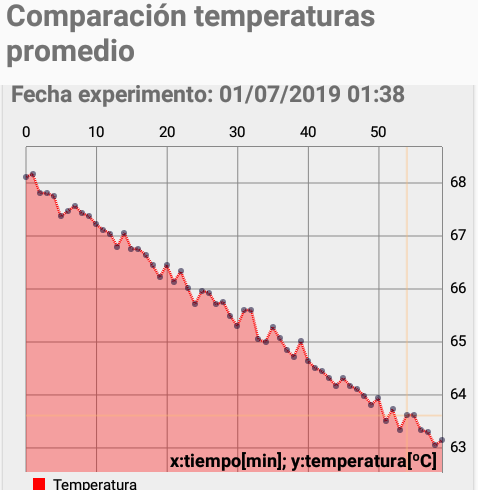
\includegraphics[scale=0.65]{Pruebas/SimpleExp1.jpg}
                \captionof{figure}{Evolución de la temperatura durante las mediciones en experimento 1}
                \label{fig:SimpTempExp1}
            %\end{figure}
    \end{minipage}     
            %Experimento 2
            \begin{figure}[H]
                \centering
                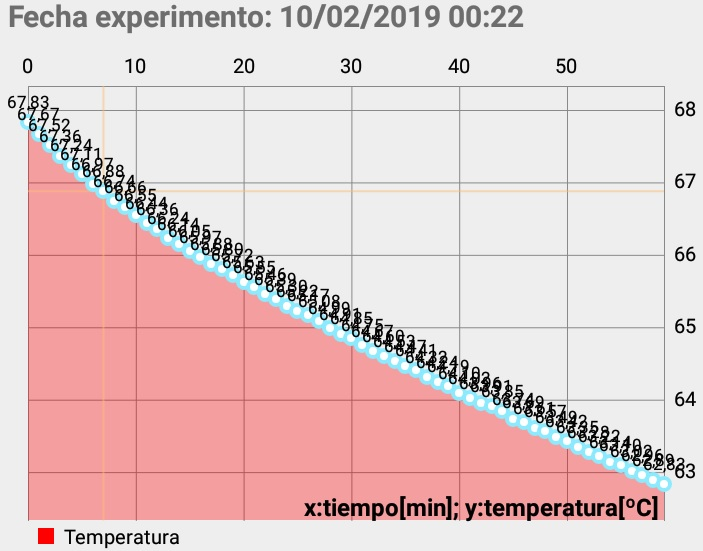
\includegraphics[scale=0.65]{Pruebas/SimpleExp2.jpg}
                \captionof{figure}{Evolución de la temperatura durante las mediciones en experimento 2}
                \label{fig:SimpTempExp2}
            \end{figure}

        %\end{minipage}
        
        %\begin{minipage}{\textwidth}
                   
           %Experimento 3
            \begin{figure}[H]
                \centering
                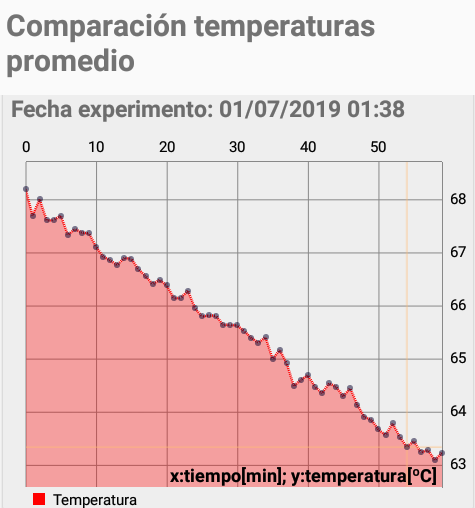
\includegraphics[scale=0.65]{Pruebas/SimpleExp3.jpg}
                \captionof{figure}{Evolución de la temperatura durante las mediciones en experimento 3}
                \label{fig:SimpTempExp3}
            \end{figure}
        
            %Valores generales/promedio
            \begin{figure}[H]
                \centering
                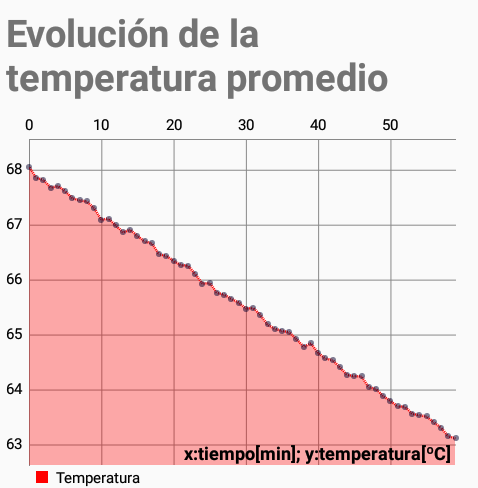
\includegraphics[scale=0.65]{Pruebas/SimpleEvolTempProm.jpg}
                \captionof{figure}{Evolución de la temperatura promedio de todos los Experimentos}
                \label{fig:SimpTempProm}
            \end{figure}
           
            \begin{figure}[H]
                \centering
                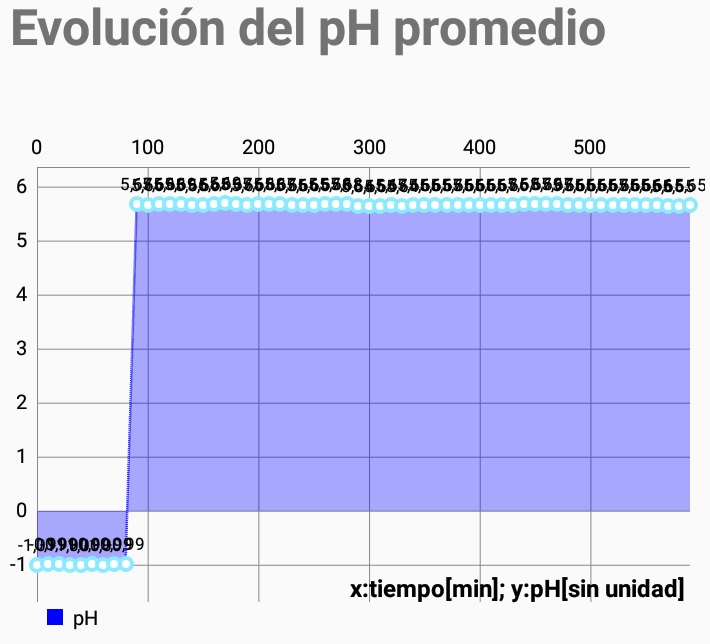
\includegraphics[scale=0.65]{Pruebas/SimpleEvolPHProm.jpg}
                \captionof{figure}{Evolución del pH promedio de todos los Experimentos}
                \label{fig:SimpPHProm}
            \end{figure}

    \section{Pilsen Lager - Escalonada}
         %Experimento 1
            \begin{figure}[H]
                \centering
                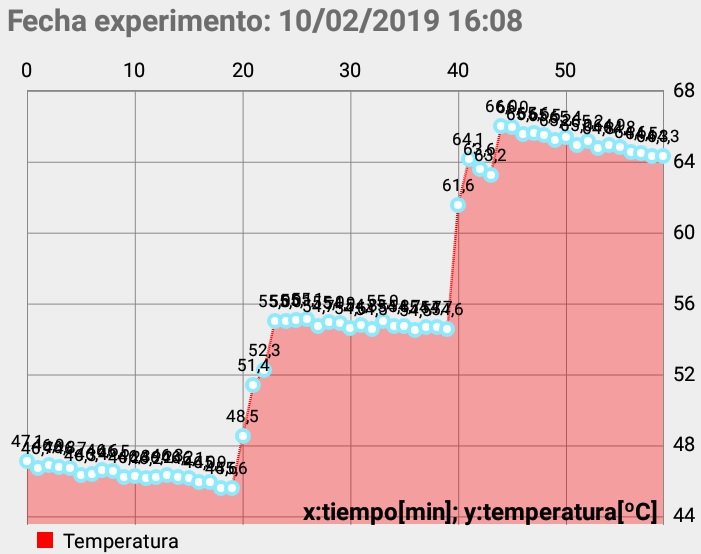
\includegraphics[scale=0.65]{Pruebas/EscalonadaExp1.jpg}
                \captionof{figure}{Evolución de la temperatura durante las mediciones en experimento 1}
                \label{fig:EscExp1}
            \end{figure}
        %\end{minipage}
        
        
            \begin{figure}[H]
            %\begin{minipage}{\textwidth}    
                \centering
                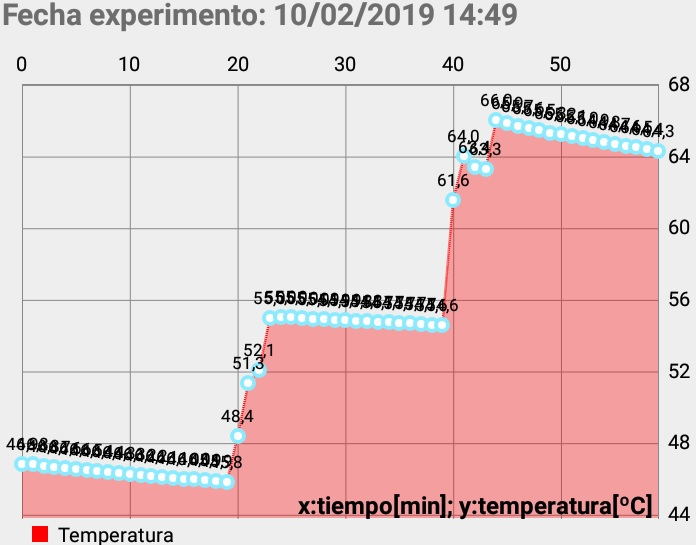
\includegraphics[scale=0.65]{Pruebas/EscalonadaExp2.jpg}
                \captionof{figure}{Evolución de la temperatura durante las mediciones en experimento 2}
                \label{fig:EscExp2}
            \end{figure}
                
            \begin{figure}[H]    
                \centering
                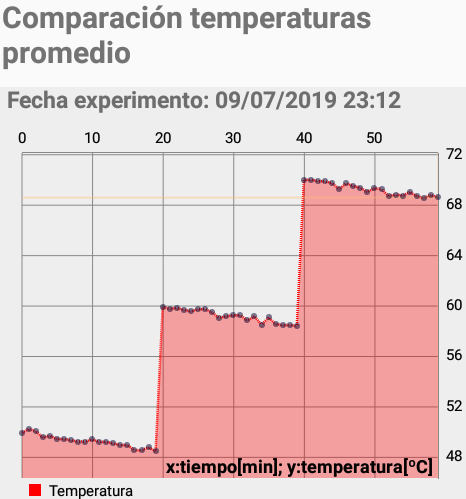
\includegraphics[scale=0.65]{Pruebas/EscalonadaExp3.jpg}
                \captionof{figure}{Evolución de la temperatura durante las mediciones en experimento 3}
                \label{fig:EscExp3}
            \end{figure}

            \begin{figure}[H]
                \centering
                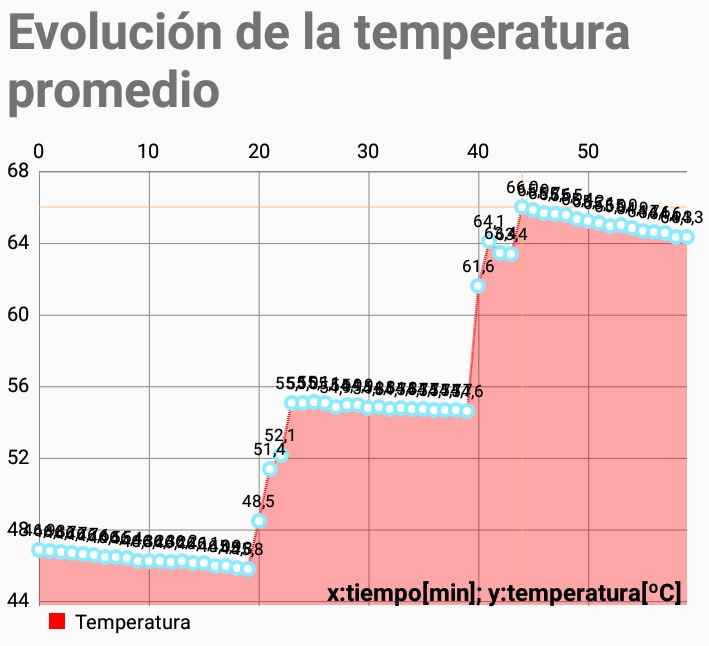
\includegraphics[scale=0.65]{Pruebas/EscalonadaEvolTempProm.jpg}
                \caption{Evolución de la temperatura promedio de todos los Experimentos}
                \label{fig:EscTempProm}
            \end{figure}
        
            \begin{figure}[H]
                \centering
                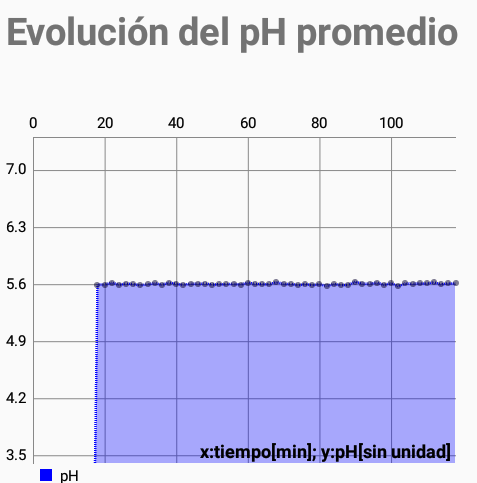
\includegraphics[scale=0.65]{Pruebas/EscalonadaEvolPhProm.jpg}
                \caption{Evolución del pH promedio de todos los Experimentos}
                \label{fig:EscPhProm}
            \end{figure}     
